\documentclass{article}

% if you need to pass options to natbib, use, e.g.:
% \PassOptionsToPackage{numbers, compress}{natbib}
% before loading nips_2018

% ready for submission
\usepackage{nips_2018}

% to compile a preprint version, e.g., for submission to arXiv, add
% add the [preprint] option:
% \usepackage[preprint]{nips_2018}

% to compile a camera-ready version, add the [final] option, e.g.:
% \usepackage[final]{nips_2018}

% to avoid loading the natbib package, add option nonatbib:
% \usepackage[nonatbib]{nips_2018}

\usepackage[utf8]{inputenc}      % allow utf-8 input
\usepackage[T1]{fontenc}         % use 8-bit T1 fonts
\usepackage[hidelinks]{hyperref} % hyperlinks
\usepackage{url}                 % simple URL typesetting
\usepackage{booktabs}            % professional-quality tables
\usepackage{amsfonts}            % blackboard math symbols
\usepackage{nicefrac}            % compact symbols for 1/2, etc.
\usepackage{microtype}           % microtypography

\title{Automatic Text Summarization \\ \normalsize{Summer Term 2018 - Group 5} \\ \vspace{1em} \large Johanna Heinz, Markus Höhn, Marcel Juschak, Lukas Raymann, Steven Lamarr Reynolds, Sebastian Seipp \\ \vspace{1em} 2018--08--07}

% The \author macro works with any number of authors. There are two
% commands used to separate the names and addresses of multiple
% authors: \And and \AND.
%
% Using \And between authors leaves it to LaTeX to determine where to
% break the lines. Using \AND forces a line break at that point. So,
% if LaTeX puts 3 of 4 authors names on the first line, and the last
% on the second line, try using \AND instead of \And before the third
% author name.

%\author{
%  David S.~Hippocampus\thanks{Use footnote for providing further
%    information about author (webpage, alternative
%    address)---\emph{not} for acknowledging funding agencies.} \\
%  Department of Computer Science\\
%  Cranberry-Lemon University\\
%  Pittsburgh, PA 15213 \\
%  \texttt{hippo@cs.cranberry-lemon.edu} \\
%  %% examples of more authors
%  %% \And
%  %% Coauthor \\
%  %% Affiliation \\
%  %% Address \\
%  %% \texttt{email} \\
%  %% \AND
%  %% Coauthor \\
%  %% Affiliation \\
%  %% Address \\
%  %% \texttt{email} \\
%  %% \And
%  %% Coauthor \\
%  %% Affiliation \\
%  %% Address \\
%  %% \texttt{email} \\
%  %% \And
%  %% Coauthor \\
%  %% Affiliation \\
%  %% Address \\
%  %% \texttt{email} \\
%}

\author{Johanna Heinz, Markus Höhn, Marcel Juschak Lukas Raymann,Steven Lamarr Reynolds, Sebastian Seipp}

\begin{document}
% \nipsfinalcopy is no longer used

	\maketitle

	% !TeX root = ..\essay.tex

\section{Introduction}
Automatic text summarization is the task of automatically creating summaries from
given text sources. For the project described in this report the process was
divided into three pipeline steps:
\begin{itemize}
    \item Step 1 - Content Selection: The task here was to select relevant
        nuggets (sentences or part of sentences) out of the input. The
        input consisted of important sentences that were extracted from
        documents and covered 49 topics.
    \item Step 2 - Creating Hierarchies: The task of this step was to create
        hierarchies that represented the structure of the nuggets from the
        previous step and ordered them into subtopics.
    \item Step 3 - Creating Summaries from Hierarchies: In the last step the
        hierarchies of the second step had to be converted into short summaries.
        The summaries could be either about the complete topic or subtopics.
\end{itemize}
Our group chose to do all three pipeline steps and create general summaries
without focusing on just a few subtopics. The implementation process and
the results will be further explained in the following chapter. In
chapter~\ref{ch:evaluation} information about the quality of the resulting
summaries are also given in the form of an evaluation.
	% !TeX root = ..\essay.tex

\section{Hierarchical Approach}

	% !TeX root = ..\essay.tex

\subsection{Step 1 - Content Selection}
In this step we dealt with choosing content from a set of given sentences and headings which is generally appropriate for a summarization. What we did can be divided in three parts. First we analyzed the data in order to gain some insights and orientate ourselves so that we know in what direction we can potentially go. After we found the general direction, we tried out four different approaches to retrieve nuggets and picked one of them. After it was fine tuned, we generated our nuggets as input to the next pipeline step.
\subsubsection{Data Analysis}
\textbf{Structure of nuggets}\\
First, we looked at how many nuggets are whole sentences. "Whole sentence", in this context, means that there is a 1:1 counterpart in the relevant sentences input file. Finding such a counterpart was actually nto trivial, since...\lbrack Manche Sätze waren doch quasi preprocessed "arent" -> "are nt", ist das Problem hier aufgetreten oder wo anders? Außerdem finde ich gerade kein Beispiel dafür, das würde ich hier aber angeben\rbrack. We solved this by using difflib \lbrack Link to website\rbrack, which gives a score of how similar two sequences (of characters) are. We chose a threshold of ???\% and declared every pair of sentences with a similarity above that threshold to be the same. As a result, we found that depending on the topic between 70.5\% to 87.9\% of nuggets are whole sentences with a mean of 82\%. This ratio was surprisingly high and led us to a big simplification we have made, which is to assume that all nuggets are always complete sentences. Therefore, the core problem we have to tackle is to decide whether a given sentence is a nugget or not.\\
We further analyzed the structure of nuggets by searching for patterns like certain words that appear primarily in nuggets or no nuggets. We thought that words like "significant" or "important" could indicate that there is relevant information content in this sentence and thus would make good features. Unfortunately, it turned out that words are very much equally distributed over both types of sentences. Which words appear most often is, as you would expect, topic dependend.
\textbf{Ratios of Nuggets}\\
Next, we analyzed how the proportions between nuggets and no nuggets are in the relevant sentences we were given as input. We found out that, depending on the topic, between 9.3\% to 24.9\% of sentences are nuggets with a mean of 14.1\%. Knowing the distribution of positive and negative examples, i.e. nuggets and no nuggets, is important, because it directly affects the learning process of the later classifier. If for example there are only 10\% positive examples,  a classifier may choose to always predict the majority class, which would be the negative one, no nugget. This leads to a high precision but is not what we want. When we know these numbers, we can multiply the amount of positive examples to reach something close to a 50:50 distribution. Hereby we would increase the cost of classifying a positive instance wrong and therefore have more control over the learning process of the classifier.

\subsubsection{training classifiers}
After gaining sufficient insight into the data we were given, we created binary labeled versions of them. For preprocessing we used gensims simple preprocess \lbrack cite/link!\rbrack .We thought about different approaches to train a classifier and ended up with four general variants.\\
\textbf{FastText}\\
FastText \cite{joulin2016bag} is an open-source library for text classification and word embeddings developed by Facebook AI Research (FAIR) lab. Since it already provides an implemenation for text classification using word embeddings, we just had to transform our data into the right format and potentially change the ratio of positive and negative examples in order to control the learning process of the classifier. \lbrack nachdem ich hier nochmal rumprobiert habe, bekomme ich Recall = 0.1617, Precision = 0.8175, was besser erscheint als es sein sollte! Was fangen wir jetzt damit an? \rbrack. Because of ... we did not trust these results?... \\
\textbf{Naive Bayes}\\
Naive Bayes was our only approach that did not involve word embeddings. As features we chose the words themselves, \lbrack did we?\rbrack , we also used the sentence length with discretized intervals and we used a POS tagger to create a binary feature of whether a verb is present or not. Unfortunately the results were very bad. That is because first of all, we did not find enough good features and second, the POS tagger could not reliably tell whether a sentence contained a verb or not.\\
This approach became interesting when we included 10 further features of which each one corresponded to one of the top 10 most frequent words in that topic and whether it is present in the sentence or not. This resulted in a recall of 37.8\% and a precision of 19.5\%, which is actually something you would be able to work with. The downside to this is, that you can train a classifier only for one specific topic and you need training data for it. So there is no way to retrieve nuggets for a topic without training data. In conclusion we can say, that this approach did not work at all.\\
\textbf{Fully Connected Neural Network}\\
In our neural network approaches we chose to represent words with 300 dimensional GloVe embeddings. In order to create a good representation for complete sentences instead of only words, we averaged the sum of all word embeddings of a sentence. We chose this representation because it does not require heavy computations and seems to still deliver good results as indicated by \cite{iyyer2015deep}. Furthermore, we decided to take into account the context of the sentence to be classified. In order to do this, the k preceding and succeeding sentences (according to the document in the input xml) are used as input as well.\\
We implemented our network with Keras and chose as parameters... . As a result we obtained a precision of 35\% and a recall of 1.5\%. In order to summarize a topic, these results are not sufficient at all.\\
\textbf{Convolutional Neural Network}\\
The architecture we chose in the end was a convolutional neural network. For this approach, we classified sentences in isolation instead of including the context and we did not represent the sentence as the average of its word embeddings but instead as a sequence of its word embeddings. We made more restrictions by excluding sentences with less than 5 and more than 50 words and padded each sentence to 50 words. We made this decision because we observed that phrases like \textit{U.S. History II}, \textit{I don't know.} or \textit{All-School Assemblies} cannot make good summaries and neither do sentences that span more than 50 words. We padded the input to 50 words because our architecture expects a fixed amount of them. We also filtered out sentences with containing phrases or characters like "I", "?", "We" in order to filter out personal opinions etc... .\\
In order to find the right parameters we conducted random search. After testing some diverse parameter configurations and got an idea of what generally works, we defined ranges for each of them. The program received these ranges, as well as the training, deveopment and validation set. It generated random configurations within the given ranges, trained the network on the training set and evaluated the model after each epoch. If performance decreased on the development set, the program finished training in order to prevent overfitting and to save ressources. If the new model beat the currently best one, it is stored and the best results are udated. Since this task is very computation heavy, we used the Lichtenberg Cluster \lbrack Link...\rbrack to do this for us. As a general restraint for the results, we decided to only allow models that have a recall of at least 5\% but a precision as high as possible. Recall and precision seem to behave anti-proportional, therefore we have to choose which one them is more important to us. Since we want to create meaningful and well readable summarizations in the end which are not very long anyway, precision is of a much greater importance to us. \\
\lbrack insert image of ranges and results of random search\rbrack \\
Our final parameters provided a recall of 5.9\% and a precision of 52\%. We noticed that for some topics \lbrack which?\rbrack the amount of predicted nuggets is very large and for some very small. This led us to the decision that we always use the 30 sentences with the highest probability of being nuggets as input to the next pipeline step. This guarantees enough material to work with in the 
later steps while using only the nuggets we are most confident in if we would have predicted more.\\
We tried improving the above results by weighting word embeddings with tf-idf weights, but they seem to only confuse the neural network. Results very terrible \lbrack what exactly did come out of this?\rbrack .\\
QUESTION: Split approach and evaluation into two parts? or discuss results directly after explaining the approach?

	% !TeX root = ..\essay.tex

% Notes from slides

% Erfolg der Methode
% 	Nutzung der Methode in der Literatur
% 	Ergebnisse auf anderen Corpora/Daten
% Literaturrecherche
% 	Erweiterungen der Methode
% 	Kritik der Methode
% Ver-/Anwendung der Methode
% theoretischer Bezug
% Praktischer Bezug
% Verwendbarkeit
% Beschreibung der Methodik
% Bewertung der Methode
% Verwendung von (Fach-)Begriffen richtig und konsistent
% Mit eigenen Worten
% Wissenschaftliches Arbeiten
% Korrekte Zitierweise
% Weiterfuehrende Ideen und Gedanken

% What is the prob­lem that the au­thors tried to solve in this paper?
% How does this prob­lem re­late to the topic of the sem­i­nar and to other talks in the sem­i­nar?
% How can I ex­plain the au­thors' so­lu­tion in the best way?
% How did the au­thors demon­strate that the so­lu­tion works?

\subsection{Step 2 - Creating Hierarchies}

\subsubsection{Introduction}

In the second step of our pipeline, we created tree hierarchies out of the sentences that were selected in the first step. The results of the content selection created a list of sentences for each topic. Our system took those sentences and created a tree with each branching tree indicating a new subtopic. Each node of a tree contained one or more sentences. At the top is a root level with multiple trees that differ in the topics of their sentences. 

The tree hierarchies are built for the third step to better distinguish between topics of sentences. Each resulting tree should contain sentences that are similar in meaning and topic. At the top of each tree should be the most general sentence and at the bottom the most specific sentence.


\subsubsection{Method}

To prepare the Nuggets for the rest of this method we removed stopwords and words with a length lower than three, tokenized the words and we stemmed the words. For a list of stopwords, tokenization and stemming we used NLTK \cite{nltk}.

Our method can be described in three steps. First, we defined a recursive function to insert a sentence into the resulting tree. Then we defined two functions to determinate where to go in the tree. These functions also implement how similarity and specific/general sentences are calculated.

\begin{figure}[H]
	\centering
	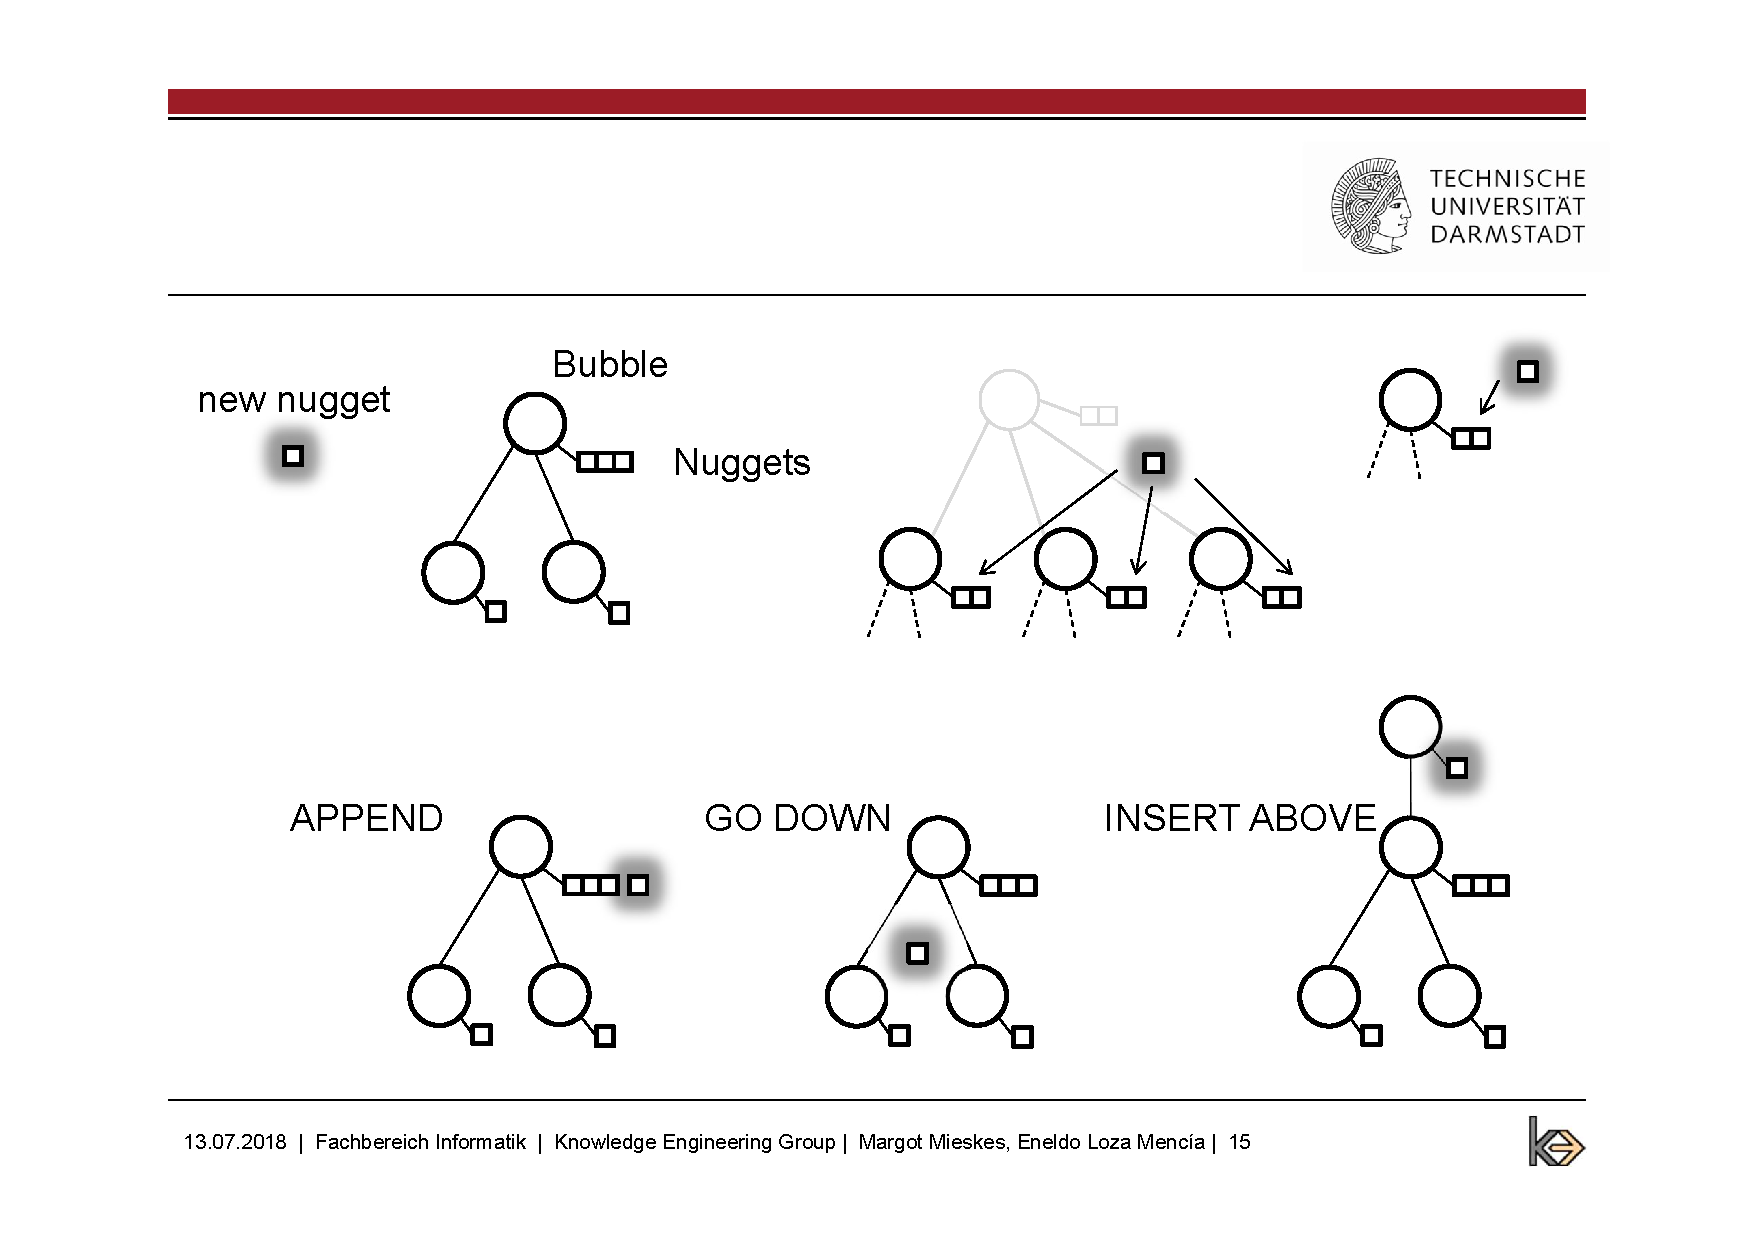
\includegraphics[trim=3cm 10cm 15cm 5.8cm, clip=true]{img/step2_func.pdf}
	\caption{new Nuggets and Bubble with Nugget}
	\label{fig:nuggetbubble}
\end{figure}
\subsubsubsection{\textbf{Insert function}}

The insert function takes a nugget and inserts it into the given tree. It runs recursively over the tree and calls the Which and Compare functions to determine where to go. Each step it first calls the Compare function which takes the current list of nuggets and the nugget which should be inserted. It returns the position where to insert the given nugget. There are three decisions to consider.
\begin{figure}[H]
	\centering
	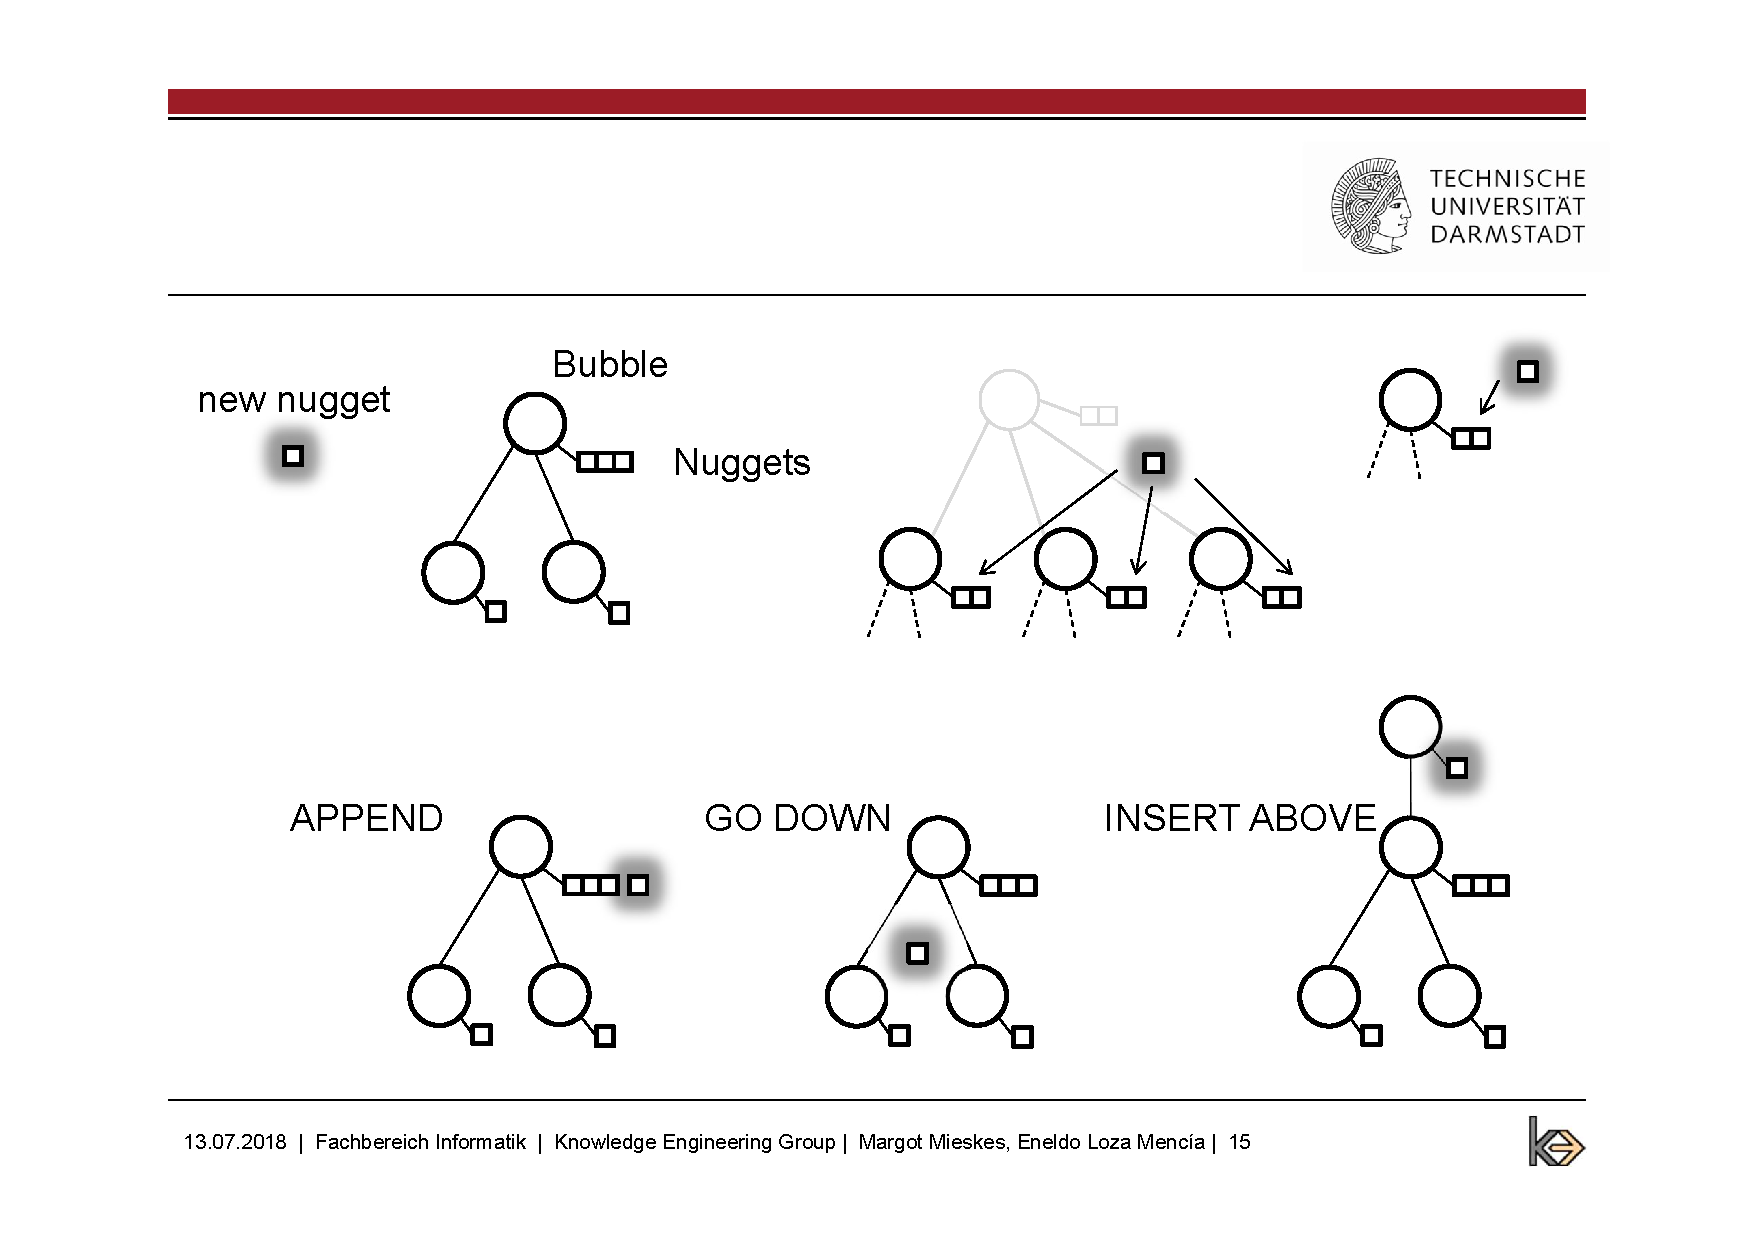
\includegraphics[trim=3.5cm 3cm 3cm 11cm, clip=true, width= \textwidth]{img/step2_func.pdf}
	\caption{Three results of Insert}
	\label{fig:insert}
\end{figure}

\begin{description}
\item [Append] It appends the given nugget to the current list of nuggets.
\item [Go Down] We call Which to determine in which bubble to go recursively. The which function returns the best Bubble to insert. The function then calls itself recursively in this Bubble.
\item [Insert Above] A new Bubble is created and inserted above the current Bubble and the pointers between the Bubbles are pointed to their new positions.
\end{description}

\subsubsubsection{\textbf{Which}}

The which function takes a list of Bubbles and the current Nugget to insert and returns the best position to insert the Nugget. This function tries to find the similarity of each Bubble to the current Nugget. Each Bubble can contain 1 to n Nuggets at the top level and multiple other in their siblings. We only take the 1 to n Nuggets in the top level and compare each word of each Nugget with NLTK path similarity.

We calculate the similarity for each list of Nuggets of each Bubble against our given Nugget. This is done by calculating the path similarity for each word of the list of Nuggets against each word of the given Nugget. We take the maximal value for each word and then take the average of the list. We take the maximum of the list and compare it against a self-defined threshold value. The higher this threshold is the more new Bubbles are created and the lower the deeper the tree hierarchy is.

The NLTK path similarity returns a score that describes how similar two words are. The similarity is calculated by taking the shortest path that connects the senses of the words. The similarity value is in the range of 0 to 1.

\begin{figure}[H]
	\centering
	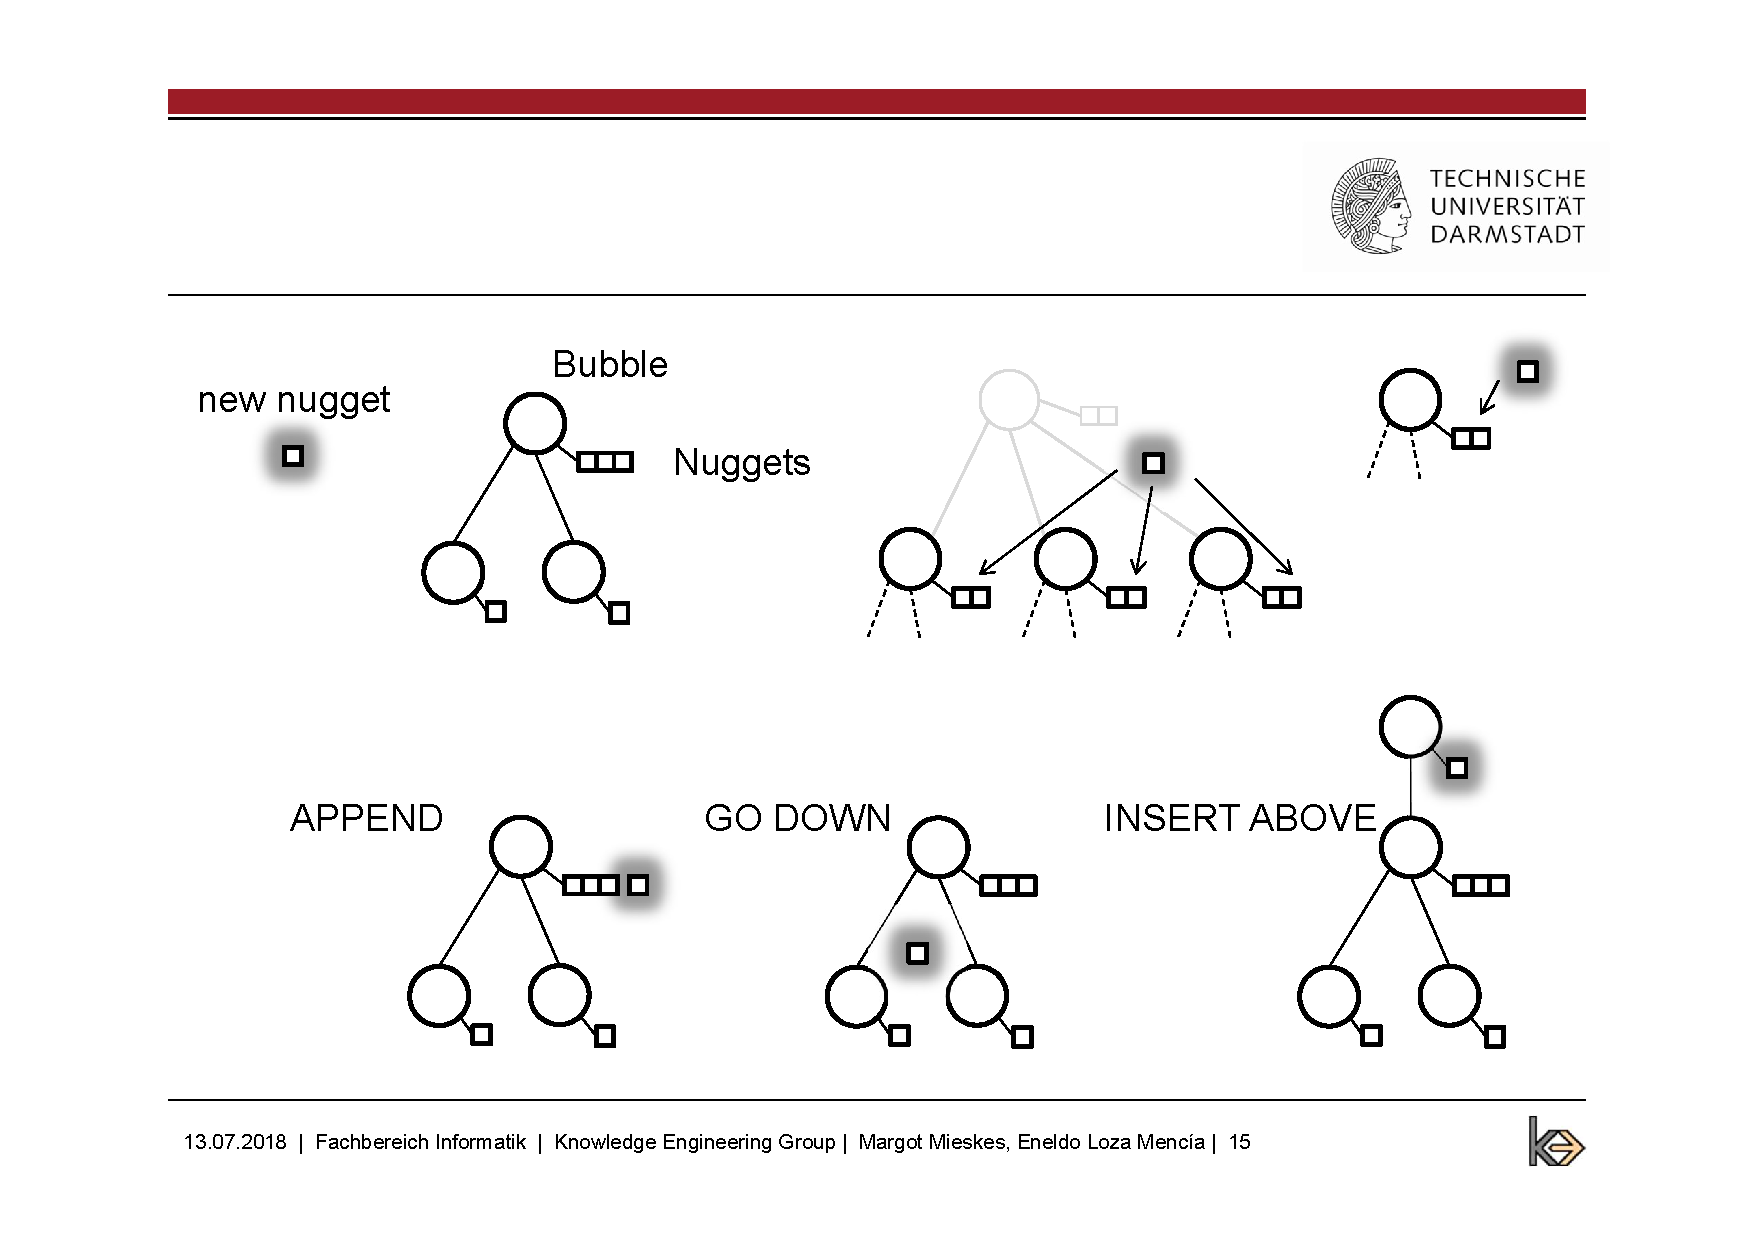
\includegraphics[trim=14cm 10cm 7cm 5.5cm, clip=true]{img/step2_func.pdf}
	\caption{Which Function}
	\label{fig:which}
\end{figure}


\subsubsubsection{\textbf{Compare}}

The compare function takes the current list of Nuggets and the Nugget which should be inserted and returns where to insert it (see list of decisions in Insert function). The goal of the compare function is to find which Nugget is more general or specific. We calculate the TF-IDF scores for the current nugget and the list of nuggets against the whole document. We do this because we want to find which Nugget is more important for the document.

TF-IDF is short for term frequency-inverse document frequency. The value increases by to the number of times a word appears in the document and is compensated by the frequency of the word in the document. This is done because some words appear more frequently in general. 

\begin{figure}[H]
	\centering
	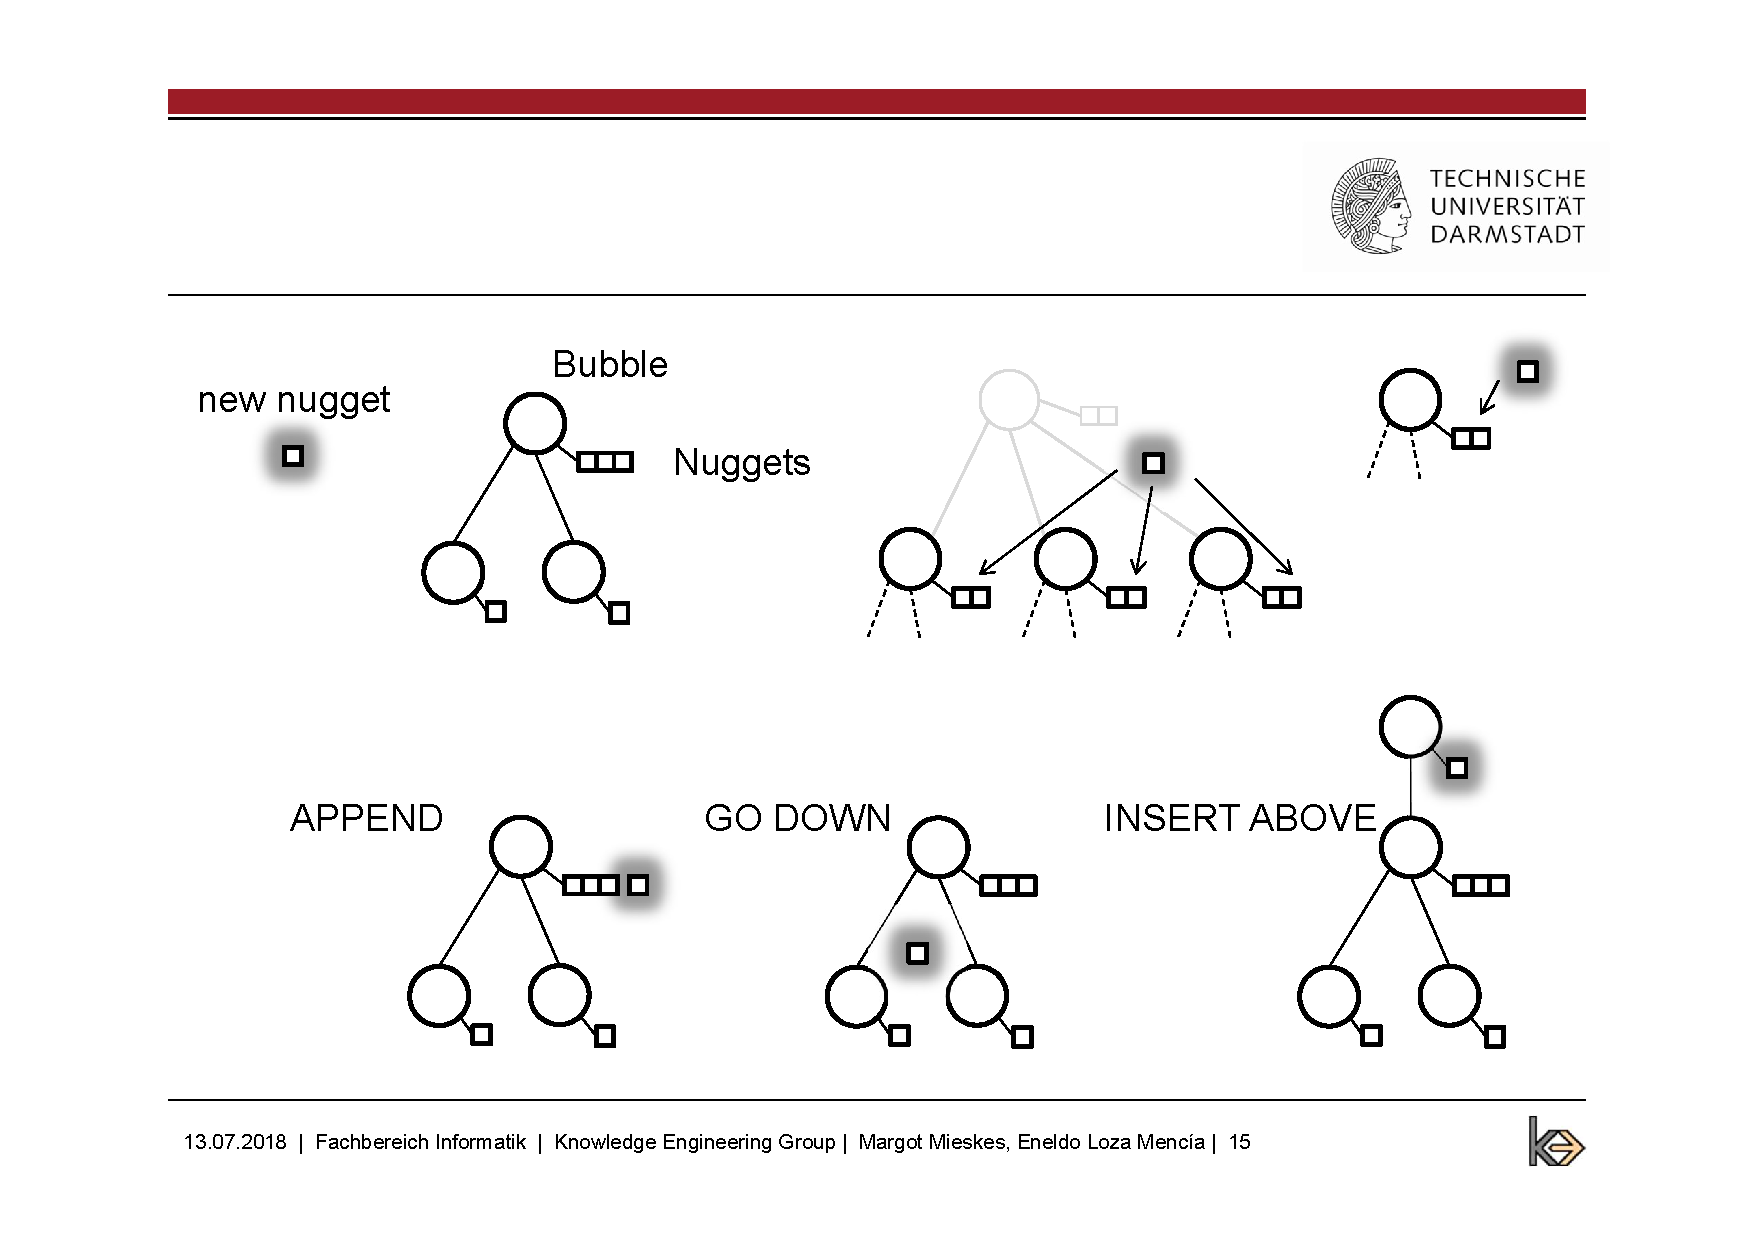
\includegraphics[trim=22.5cm 12.5cm 2.5cm 5.5cm, clip=true]{img/step2_func.pdf}
	\caption{Compare Function}
	\label{fig:compare}
\end{figure}


We thought about how we could improve our method and figured that an initial sorting of the Nuggets would help. This is already provided by the content selection of step 1. The best Nuggets appear at the beginning of the list. These Nuggets should be at the top of the hierarchy. We removed the Insert Above step from our insert function so that no Nuggets are inserted above. The Nuggets at the beginning of the list are now at the top of our hierarchy and the Nuggets further from the top are inserted deeper into the hierarchy. After we did this the quality of our resulting trees improved.

\subsubsection{Experimental Results}

For the evaluation of the hierarchies, we used the \textit{Annotation Tool} from AIPHES \cite{Tauchmann.et.al.2018.LREC}. This tool was recommended in the lecture and can compare hierarchies against each other. It displays tree similarity of two given hierarchies and against random trees. It also shows network statistics such as the number of subtrees, subtree depth, average depth, total number of bubbles and average branching.

We first used the result of our method against the given gold standard. An issue was that our hierarchy only consists of 30 Nuggets instead of the 100 to 1400 Nuggets in the gold standard. We were not sure how this changes the result of the Annotation Tool. The results showed an average of 35 percent similarity. See figure \ref{fig:graph30} for the plotted similarity of the 10 topics.

\begin{figure}[H]
	\centering
	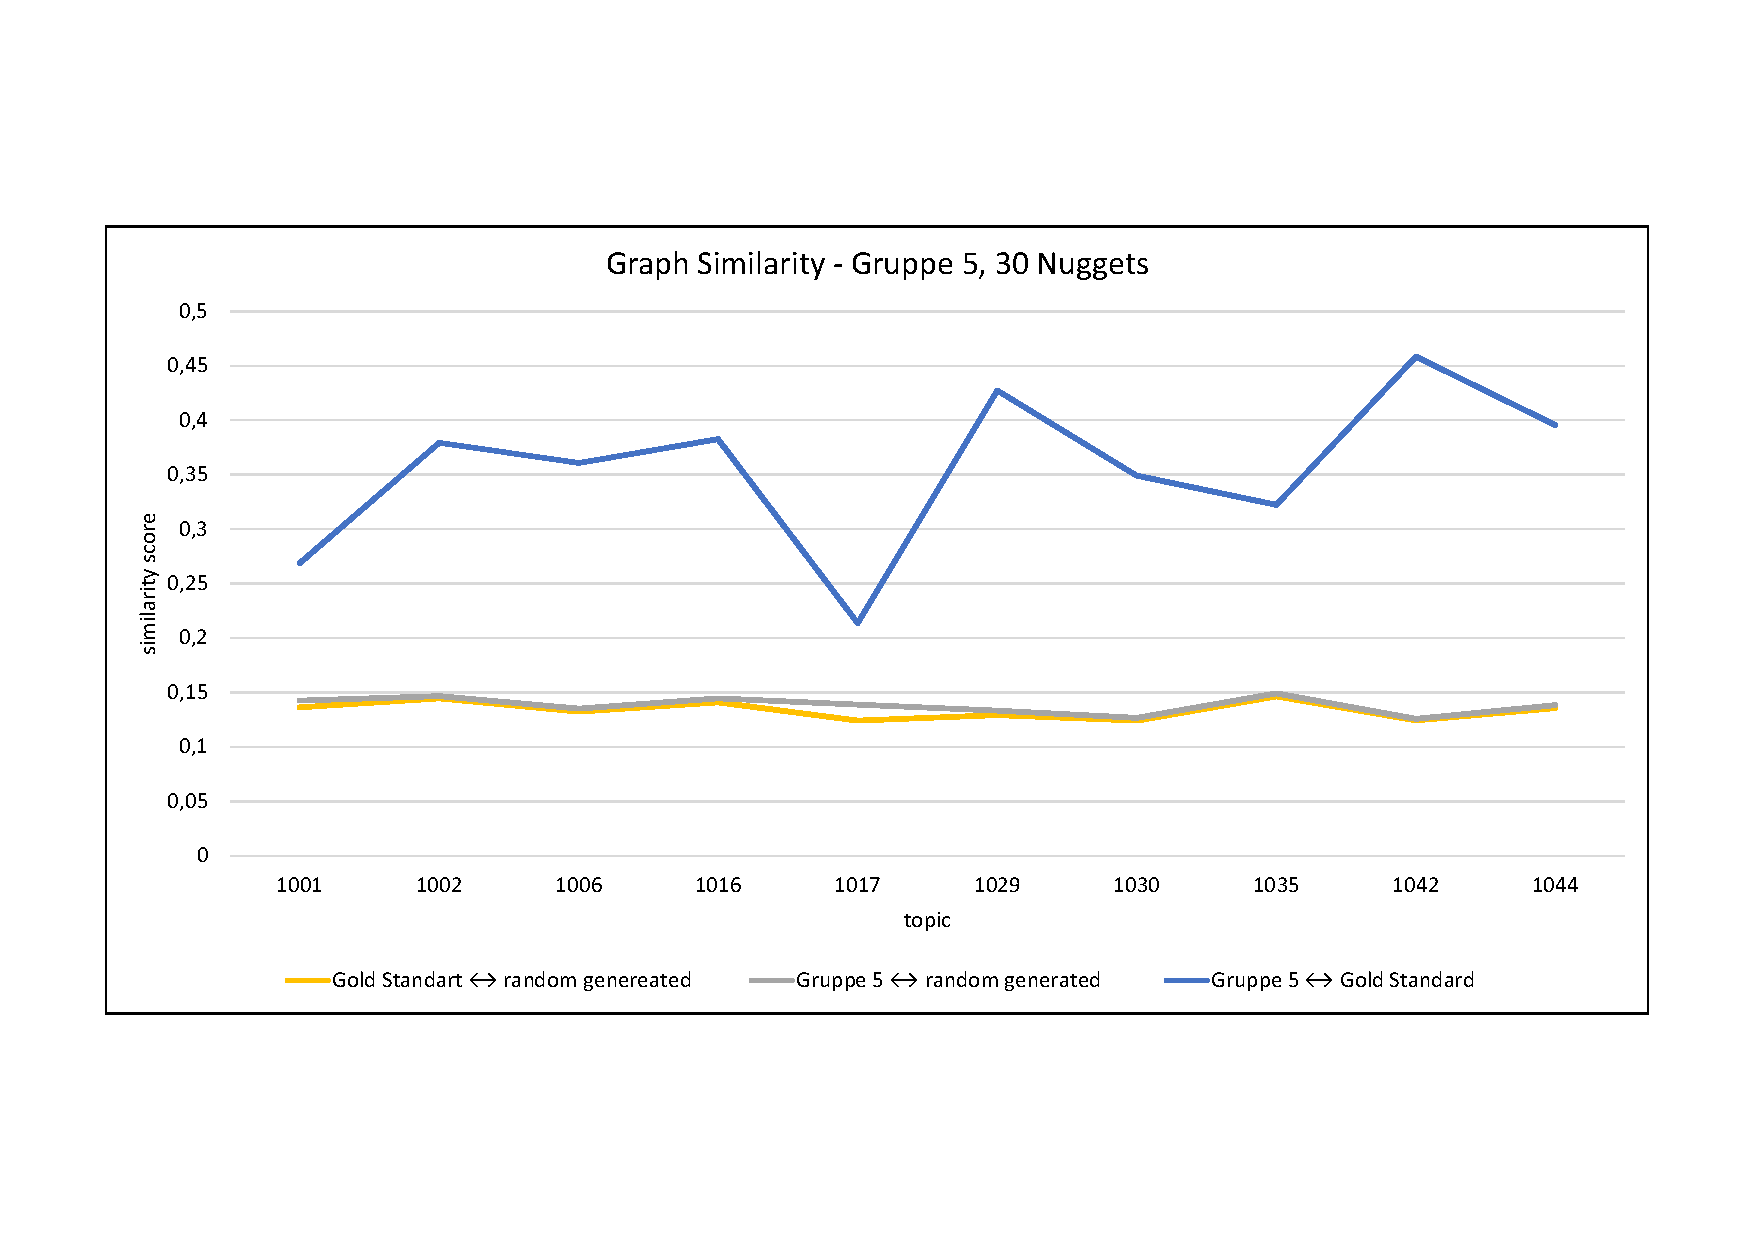
\includegraphics[trim= 0 130 0 130,width=\textwidth]{img/sim_v1.pdf}
	\caption{Graph Similarity with 30 Nuggets}
	\label{fig:graph30}
\end{figure}

We then ran our algorithm with all Nuggets to see how this changes the output of the \textit{Annotation Tool}. The issue here is that these Nuggets were not sorted by the content selection of our pipeline. The sorting of the Nuggets plays a major role in how our tree is built since we removed the Insert Above step.

The result can be seen in figure \ref{fig:graphn}. The similarity values of all three comparisons are very close. We concluded that the similarity is only noise and the trees differ too much.

Because our algorithm took a long time (up to 1 hour for one topic) for all Nuggets and the results were difficult to interpret, we could not use this evaluation intensively to improve our method. Instead, we tried to find a good balance for the number of Nuggets in each Bubble and the number of Bubbles in the root node. We applied a smoothing for the compare function to decrease the TF-IDF score when more Nuggets are present in the Bubble. This helped to increase the quality of our hierarchies.

\begin{figure}[H]
	\centering
	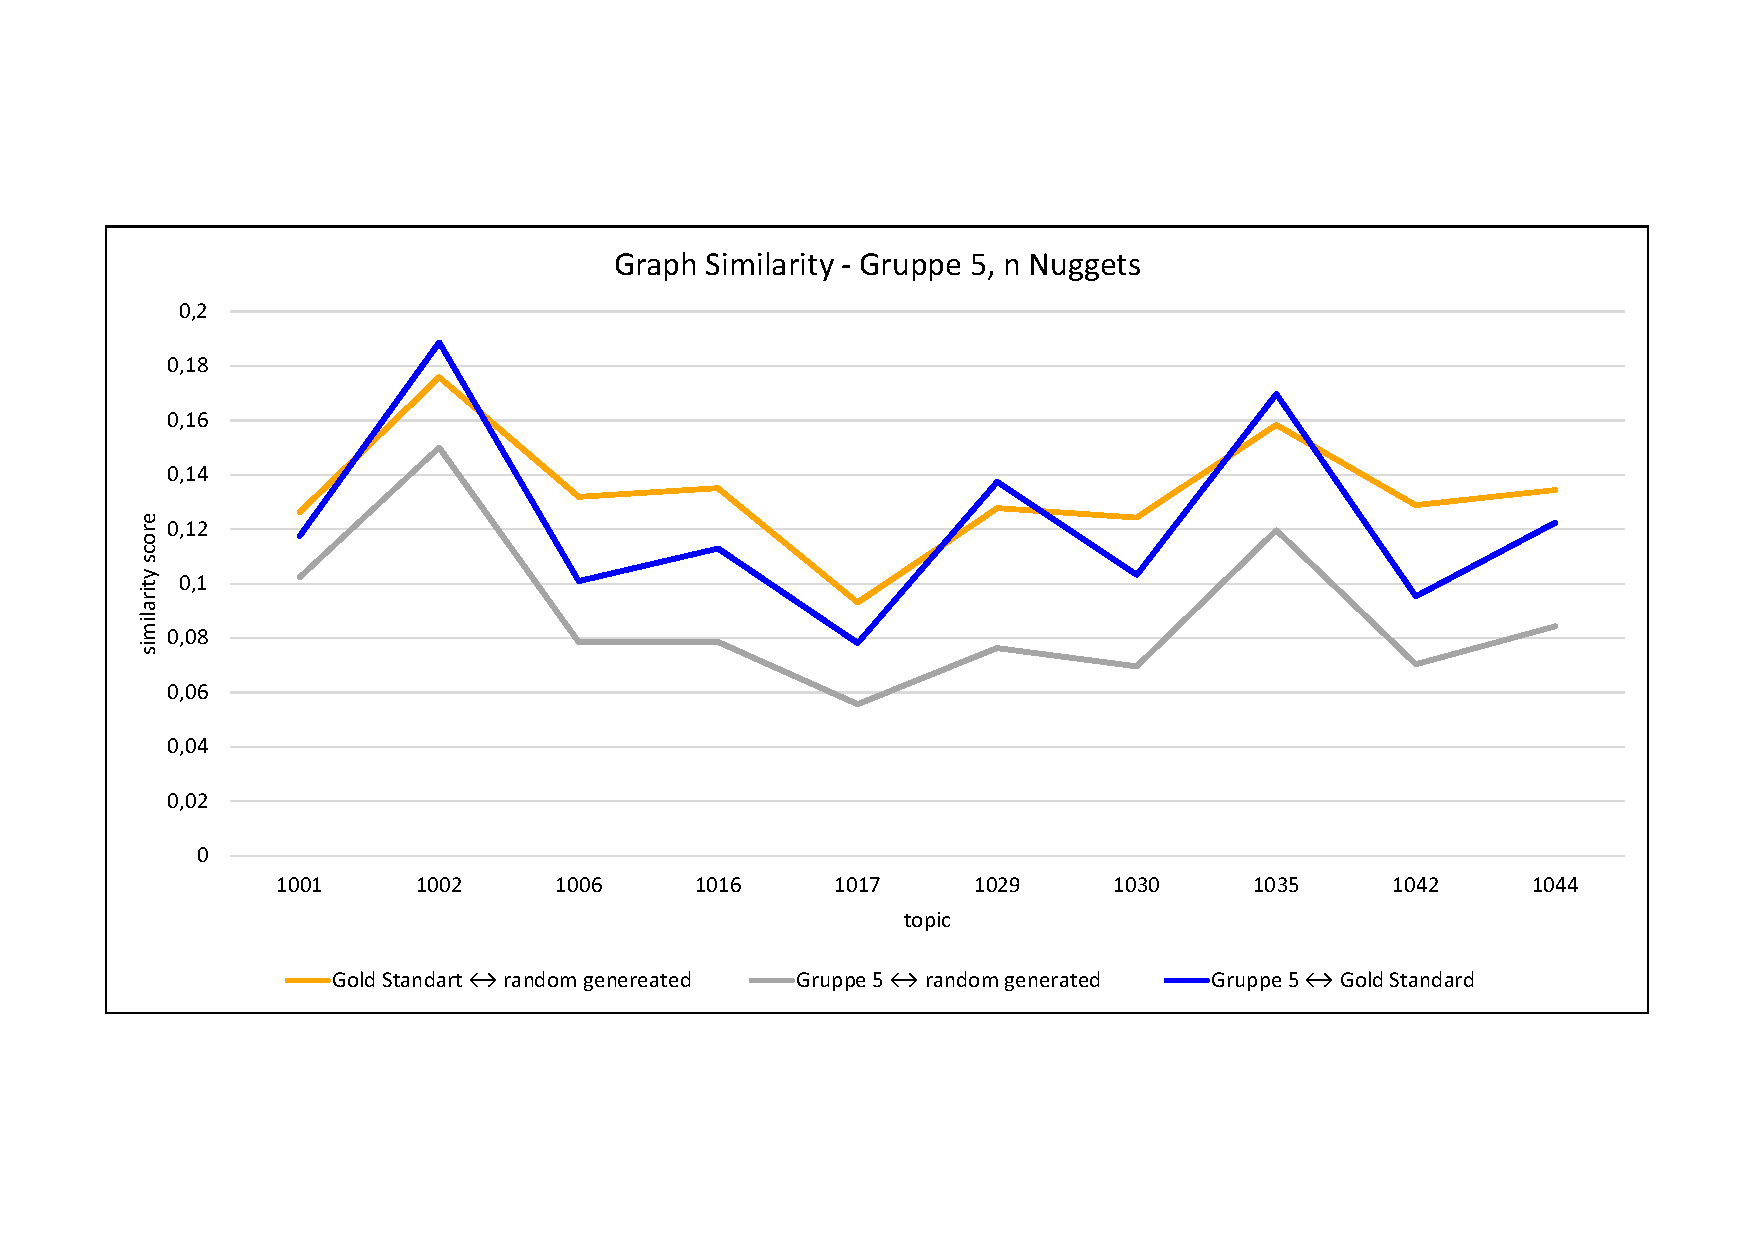
\includegraphics[trim= 0 130 0 130,width=\textwidth]{img/sim_v2.pdf}
	\caption{Graph Similarity with n Nuggets}
	\label{fig:graphn}
\end{figure}



\subsubsection{Discussion}

% hard to do an evaluation of performance on the system

% Is there a best (gold standard) hierarchy?
% Problem: How to define similarity of hierarchies?


This method can be easily improved by improving the two given functions which improve the overall system. For example, word embedding could be used to find similar Nuggets for the Which function. A clustering algorithm could be used to pre-sort the Nuggets into trees before inserting them. The compare function could be improved by using another term-weighting scheme or combining multiple.


% TODO: hard to define similar when we want general or specific

\subsubsection{Conclusions}

Our hierarchical ordering consists of three major parts. The recursive insert function, the Which function to determine where to insert a Nugget and the compare function to determine the position to insert the Nugget. We tested our method with the AIPHES \textit{Annotation Tool} and evaluated the results.
	% !TeX root = ..\essay.tex

\subsection{Step 3 - Creating Summaries from Hierarchies}
After the second step of the pipeline our system will have constructed hierarchies, as explained in the previous chapter. Each hierarchy file contains the relevant sentences of one of the topics. The hierarchies themselves consist of XML trees which should represents subtopics of the topics. The bubbles, which are nodes of the trees, can have multiple nuggets, which in our system are always complete sentences.

The task of the third pipeline step was now to construct summaries out of these hierarchy files. We focused on creating general summaries over the complete topic instead of only focusing on subtopics. 

The challenge is here the length of the summaries, because they should contain only about 600 characters. It is therefore important to select representative sentences and arrange them in a meaningful way, so that the end result has a high quality. 

Because our system uses complete sentences as nuggets, grammatically and spelling
where not a big problem, at least when the source texts were written well.

The first thing we concentrated on was to select sentences in a way that the structure of the summary feels natural and focused. To achieve this we arrived at the concept of traversing a hierarchy tree and it's nuggets in the same way a depth
first search would do it.

The idea behind this approach is that it resembles the way a human would talk about topics and subtopics. It starts with a really general
explanation of a topic and becomes more and more specific, before than switching to other subtopics, becoming there more and more specific and doing the same for other subtopics. This structure feels natural, since a human would not randomly jump between subtopics in a summary, but elaborate them one after another. When relevant sentences were selected in the first step of the pipeline and the end result of the second pipeline step has a high quality and therefore a good structure of the sentences, our summaries would automatically
also be really good.

During the development we first tested the third step with the given 10 gold standard hierarchies of the corpus, since the other steps were not completely implemented yet. Here the result was of course especially good, because the hierarchies of the corpus were done by three human annotators instead of computer-generated. When we later used the automatically generated hierarchies of our previous pipeline steps, the result thankfully still seemed to be acceptably good, which proofed the quality of the other pipeline steps.

The challenge was now of course to create summaries that had only a specific length. We cut the deeper bubbles of the hierarchy until the nuggets would sum up to the requested summary length. This means that the summaries would still contain the general information about the subtopics but not became
as specific about each.

After it was revealed that the amount of characters per summary should not be
higher than 600, which depending on the sentence length most of the time
corresponded to about 4 to 8 sentences, our approach had to be changed because such very short summaries would result in the depth first search only looking into one subtopic, and even
there just in the general nuggets, without reaching the other subtopics.

Our new approach was then to order the trees according to their size and selecting from the largest trees nuggets of the roots. The idea behind this is that a large tree size (measured by the amount of nuggets in the tree) means that the subtopic represented by this tree contains a lot of information and should therefore be included in the summary. From each tree root we selected the shortest sentence and included it into the summary. By doing this we could cover more subtrees and had therefore a wider range of information that could be covered. Selecting the sentences from the roots was done because for such a short summary it would not make sense to go into detail and take sentences from deeper within the hierarchies. 

This new approach still resulted in good summaries. They where unfortunately not as much focused and
good structured anymore as before, because they jumped from subtopic to subtopic but for a short summaries about the complete topic this is of course unavoidable.

Now that we had created our first relatively simple baseline summary we tried using some of the recommended tools to figure out if we could gain any advantage from them regarding the n the end rated criteria that will be further explained in section 3.1. These tools will automatically create a summary out of a given text each of them based on a specific algorithm. 

To obtain the input text we went a step back and created a continous text out of all the nuggets contained in the hirarchy by concatinating them according to the way a depth first search would traverse the individual bubbles. In doing so we could give the tool the complete information that was classified as relevant and extracted in step 1 and provided the possibility that the tool could take important sentences from deep down in the hirarchy that would not have made it into the summary by using the approach that created our fist baseline. It should be mentioned that the input text was exactly the same for all the different tools so that each of them would start summarizing under equal preconditions and we could better compare the created summaries against each other. 

Unfortunately, would all of the tools limit the length of the result summaries either by taking a specific word count the final summary should not exceed or by shortening the input text to a specific ratio but not one of them was able to restrict the length based on a character count. 

To tackle this problem we set the word count for each tool to an amount so that the output summary would contain approximately 600 characters. Afterwards we would cut those sentences leading to more than the demanded amount of characters. Since doing so would sometimes lead to summaries consisting of only two sentences or having a character count of only 400 or less we started adding additional sentences from our hirarchy in a similiar way we did when we created our first baseline summary. This means that we would take the shortest sentence from every root bubble, order the subtrees according to their size and select the shortest sentence per bubble from the largest subtrees untill the maximum of 600 characters was reached.

This approach had the upside that the information content of our resulting summaries was significantly improved. However, since the last sentence of the summary that was produced by one of the tools was usually more specific on a subtopic and came from deeper down in the hirarchy going back to the more general sentences of the top level bubbles would also sometimes lead to a downgrade in coherence and structure which leaves room for future improvement.  

The first tool that was examined was the the summarizer of the gensim library created by \citet{rehurek_lrec} which implements its own version of the popular graph-based TextRank algorithm to extract the most important sentences in a text. In its original form this algorithm creates a graphic representation of the input text where the sentences are its nodes and uses a measure of how much content two sentences share as a similiarity function to create edges between them. The tool however instead of implementing the original TextRank makes use of one of the proposed variations of the similiarity function (BM25) that is utilized in constructing the graphic representation of the input text from the work of \citet{DBLP:journals/corr/BarriosLAW16}. 

Unfortunately, this did somehow not work well with our input at all resulting in summaries that even though they were grammatically and spelling wise correct were neither well structured and coherent nor especially focused and jumped from subtopic to subtopic in an uncoordinated way.  

Since we could not benefit from the gensim summarizer in any way we moved on and tried making use of the sumy library created by \citet{sumy}. This library contains various implementations of different algorithms that can be helpfull for the task of summarization. Due to the fact that there were so many different implemented approaches to summarization that we tested and going into detail for each one would be to long for this report we will list all of them with a short explanation of how they generally extract the important sentences from the input text respectively: 
\begin{itemize}
	\item \textbf{Luhn:} extracts salient sentences of an input text using features like high frequency words or phrases (thereby ignoring stopwords) and how often these appear in a sentence
	\item \textbf{Edmundson:} uses key phrases in addition to frequency based weights with three methods of determining the sentence weight: first, based on presence or absence of cue words in a cue dictionary. Second, sum of all content words content words appearing the title and headings of the text. Third, location of the sentence (i.e. sentences in the beginning of a text or paragraph are more important)
	\item \textbf{Kullback Leibler divergence:} a measure of difference between the true probability distribution of words of the input text and the approximated probability distribution of the summary; sentences are greedily added as long as they decrease the KL divergence since a lower value indicates that the importance of words in input text and summary is more similar
	\item \textbf{Latent Semantic Analysis:} first a matrix with unique words in rows, sentences of the input text in columns and cells containing the number of occurences of the word in the sentence is created; afterwards this matrix is transformed into  three matrices (word x concept, diagonal matrix with scaling values, sentences x concepts) through Singular Value Decomposition which is able to extract concepts of words; finally, you can take the sentence with the highest similiarity score per concept (e.g. computed with cosine similarity) from the transposed sentence x concepts matrix into the result summary 
	\item \textbf{TextRank:} builds a graphic representation of the input text as seen above and extracts themost important sentences by running the PageRank algorithm	
\end{itemize} 
Especially the approach using the Kullback Leibler divergence and the one using Latent Semantic Analysis produced acceptable output. However, both had the problem that the created summaries usually contained a good amount of information but would also often contain sentences with pronouns or names of unfamiliar people and thus lack in terms of refenrential clarity, focus and coherence. 

Because we were not fully satisfied with the results of any of the available implementations of the sumy library we continued searching for a tool that would work well with our input and eventually discovered the summa library with its own summarizer. Once again a version of the TextRank algorithm was implemented by this tool taking BM25 as the similiarity function for creating a graphic representation of the input text according to the work of \citet{DBLP:journals/corr/BarriosLAW16}. 

Despite the poor performance of the gensim summarizer which implemented a very similar version of the TextRank algorithm this most of the time produced very good summaries that were not only well focused, structured and coherent on the one hand but had a good information content on the other hand. Why this worked so well while the gensim summarizer did not we still have to figure out. Nevertheless, became those summaries our final state due to their good overall quality.  
 
Finally, we made the observation that there were multiple sentences of the form "X \textbf{is a} short explanation of X" (e.g. "ADHD is a brain-based disorder where the chemistry of the brain (neurotransmitters) is not functioning as it should.") for several of the topics. We extracted those so called "definition sentences" through a simple matching of the strings "is a " and "is an " for every topic and added them (if there existed such a sentence in the documents) as the first sentence of the corresponding summary. This did very much improve the structure on the one hand as well as the readabilty of our summaries on the other hand since it was now clarified what specific topic a summary was all about and shortly explained said topic in its beginning.

	% !TeX root = ..\essay.tex

\section{Evaluation}
\label{ch:evaluation}

\subsection{evaluation setting}
To evaluate the summaries they were manually annotated.
Each summary has been annotated by at least four raters with the following criteria:
\begin{table}[H]
	\begin{tabularx}{\textwidth}{l|X} \toprule
		criteria & description \\ \midrule
		Grammaticality      & \\
		Non-Redundancy      & \\
		Referential Clarity & \\
		Focus               & \\
		Structure           & \\
		Coherence           & \\
		Readability         & \\
		Information Content & \\
		Spelling            & \\
		Length              & \\
		Overall Quality     & \\ \bottomrule
	\end{tabularx}
	\caption{evaluation criteria}
	\label{tab:evacriteria}
\end{table}

The score for each criteria was set with the help of a five-point Likert scale.
For each criteria the opportunity to give an estimation in weighting and confidence was be expected, too. These further possibilities to rate a summary are also realized with a five-point Likert scale.
In table~\ref{tab:evalikert} the scales for Score, Weight and Confidence are shown:

\begin{table}[H]
	\begin{tabularx}{\textwidth}{l|XXX} \toprule
		Scale & Score & Weight & Confidence \\ \midrule
		1 & very poor & completely unimportant & very low \\
		2 & poor & unimported & low \\
		3 & barerly acceptable & indifferent & half sure \\
		4 & good & important & high \\
		5 & very good & absplutely important & very high \\ \bottomrule    
	\end{tabularx}
	\caption{Likert scale for Weight and Confidence}
	\label{tab:evalikert}
\end{table}

The annotators had also the opportunity to comment each criteria for each summary with free text.

\subsection{JSD}
To compare the contents of our summaries with the source documents we used the
Jensen Shannon divergence, which we computed with \textit{SIMetrix}, a tool of
Annie Louis \citep{louis}. The scores are generated by considering the vocabulary
distributions of the summaries and the source documents. We cleared the summaries
and original texts of all HTML tags and summary titles and did the same
with the summaries of the other groups and the summaries of the first baseline
that was given to all groups. The result of the tools can be seen in
figure~\ref{fig:jsd}. Note that higher Jensen Shannon divergence scores indicate
summaries of lower quality. As can be seen our values are the third best after
the scores of group 4 and 3.
\begin{figure}[H]
	\centering
	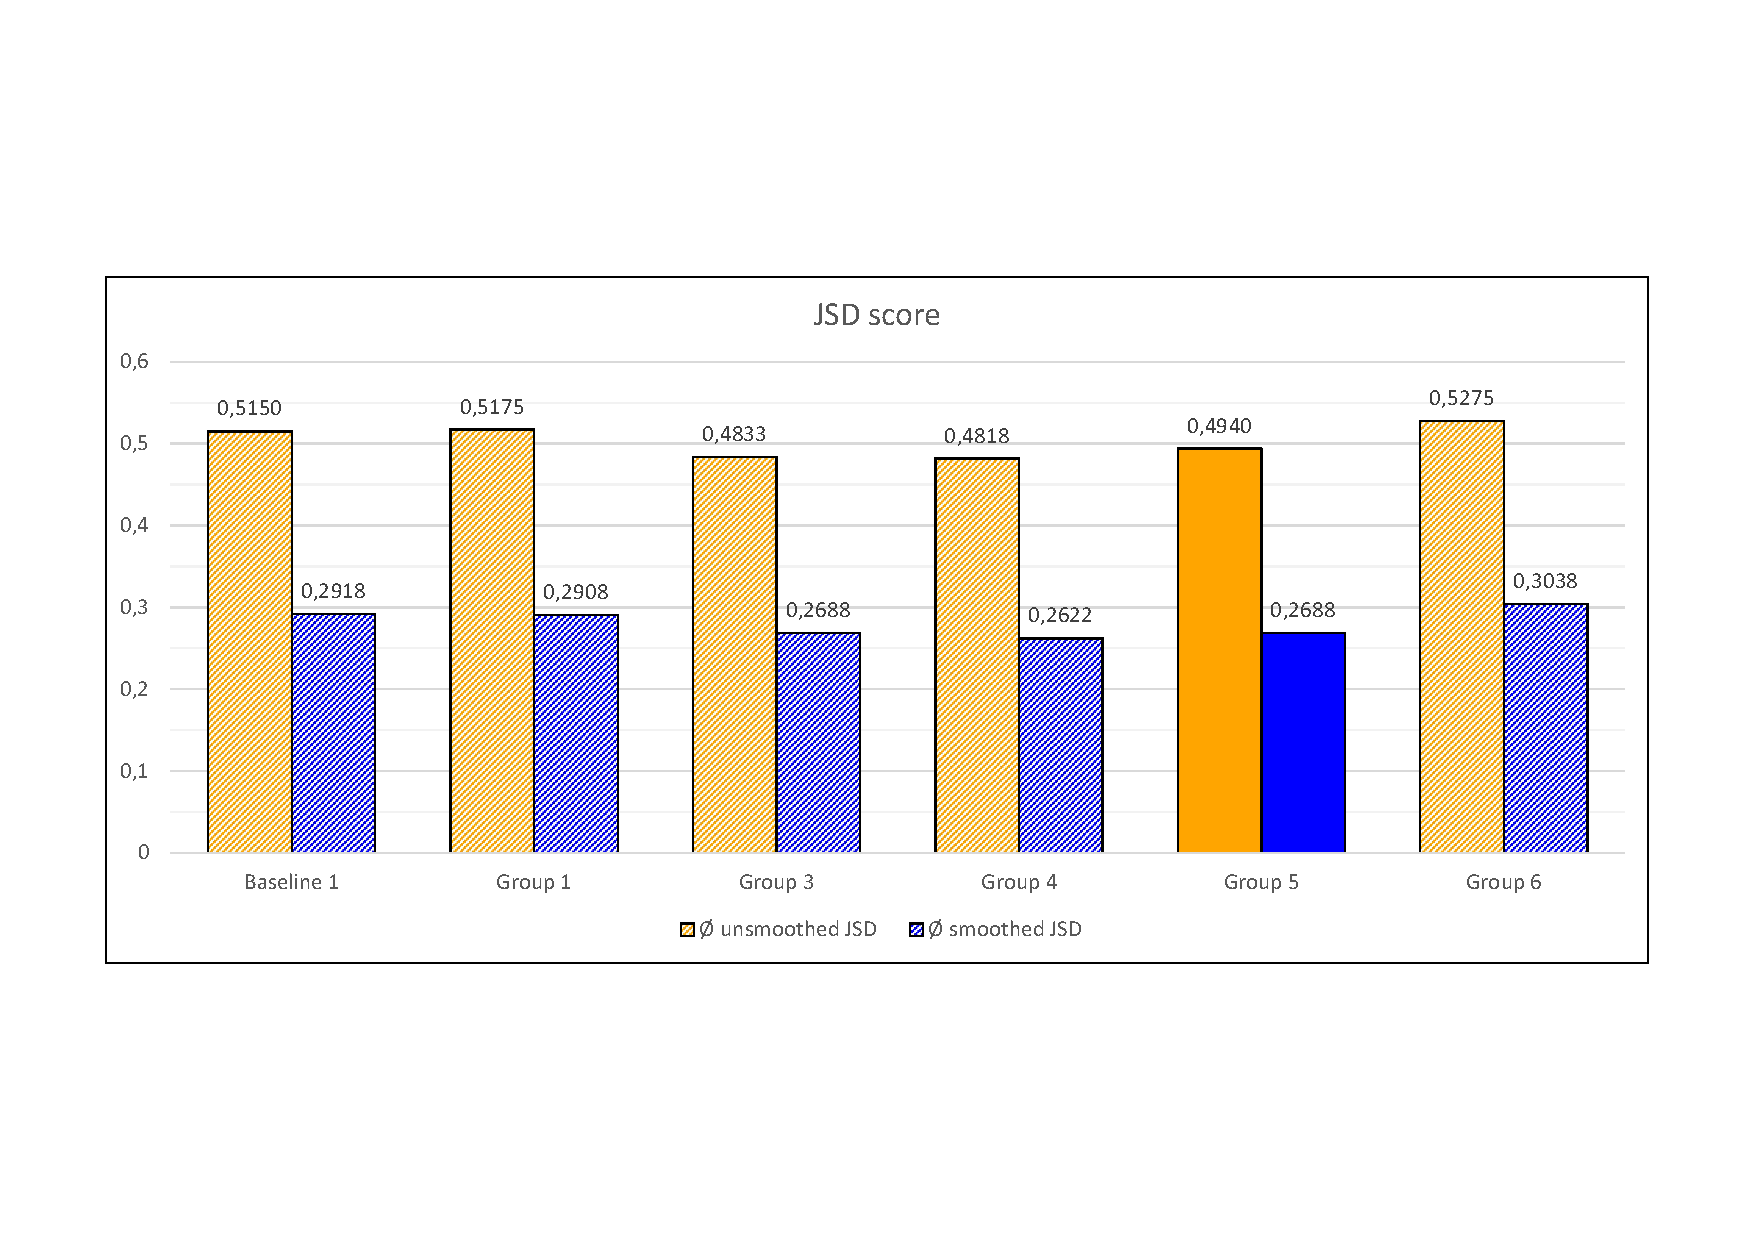
\includegraphics[trim=0 150 0 150, width=\textwidth]{img/jsd.pdf}
	\caption{JSD score}
	\label{fig:jsd}
\end{figure}


\subsection{Scores per Criteria}

First we analized our average score per criteria against the average score per critera over all groups. The results are shown in figure~\ref{fig:spc}.

\begin{figure}[H]
	\centering
	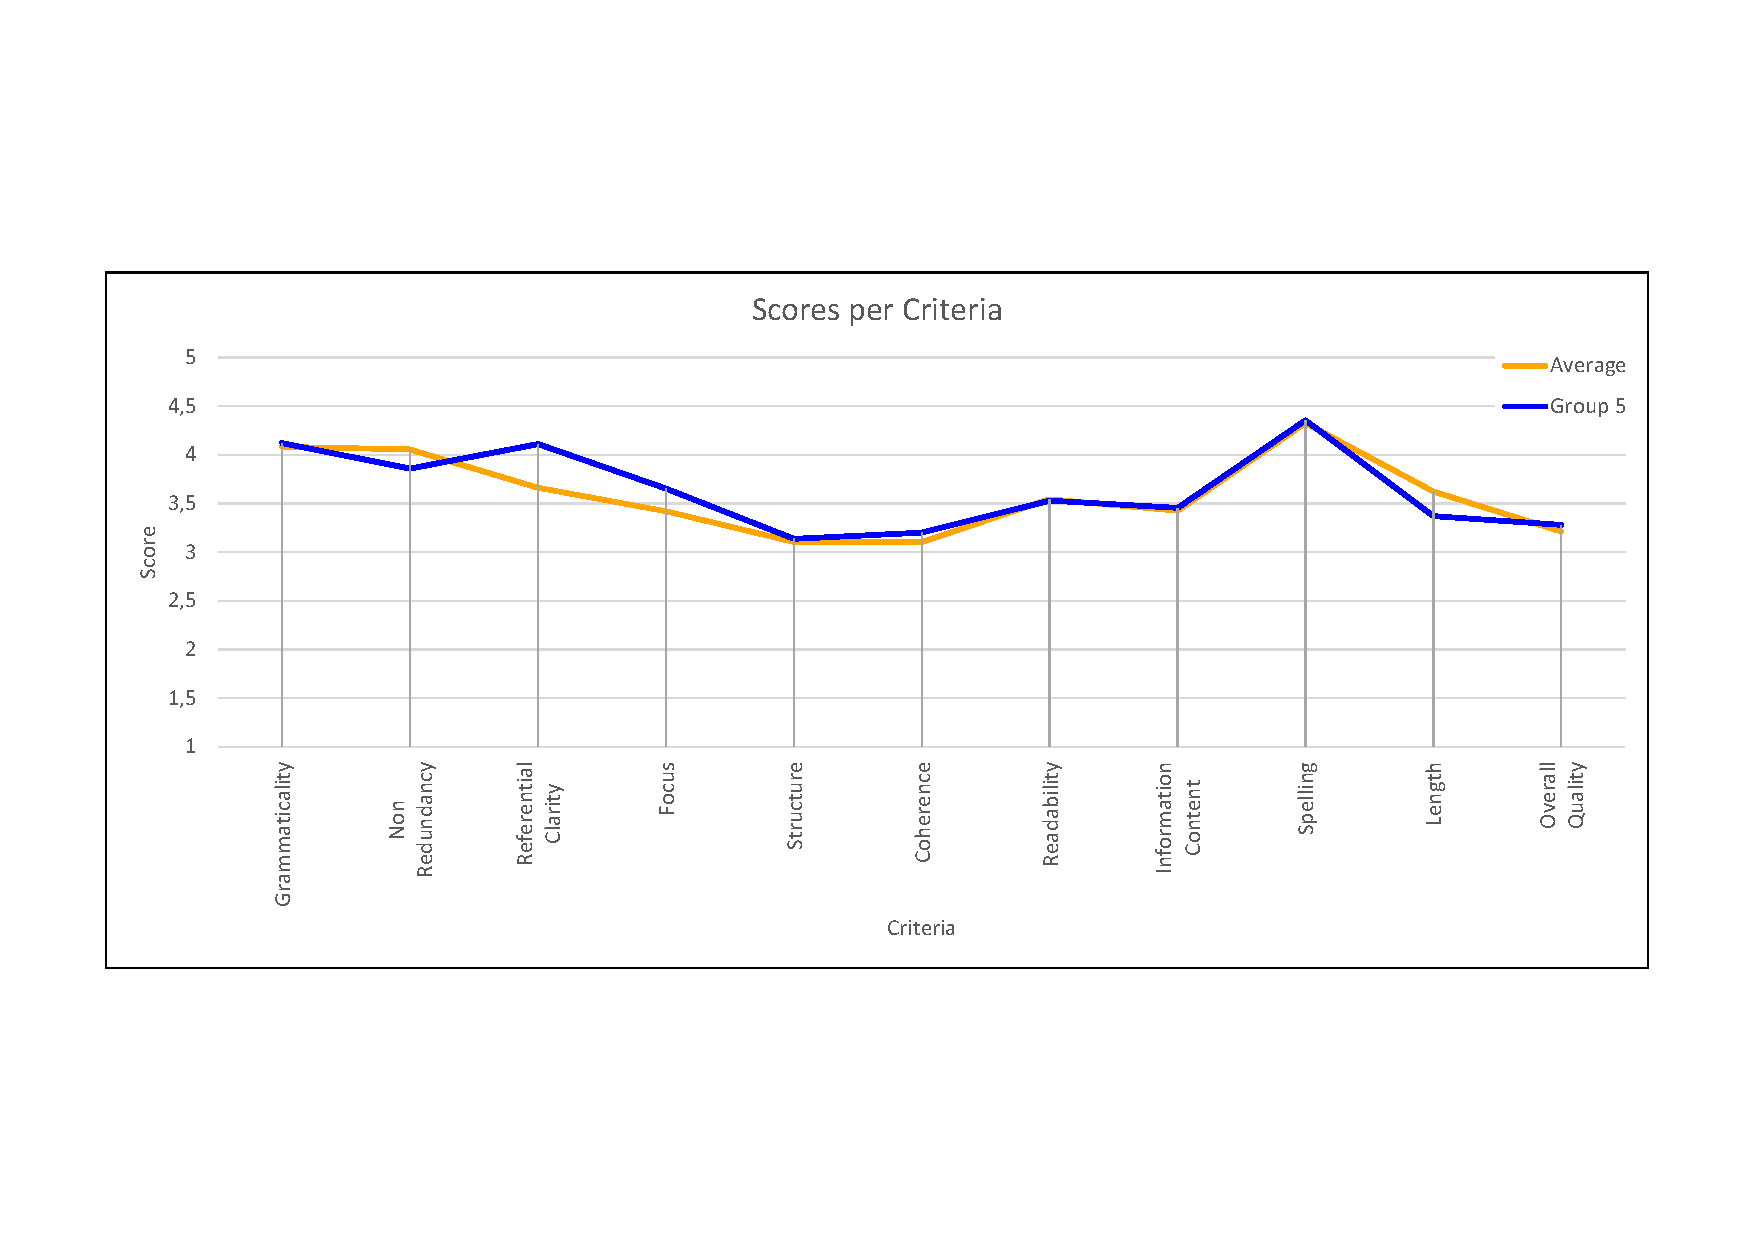
\includegraphics[trim=0 150 0 150, width=\textwidth]{img/scores_per_criteria.pdf}
	\caption{scores per criteria}
	\label{fig:spc}
\end{figure}

There are only two criteria our group is signifiant worse than the average, "non-redundancy" and "length". On the other hand there are several criteria we are better than the average, e.g. "referential clarity" or "focus".

For a better understanding of these values, we have to make a closer look at the free text comments.
In table~\ref{tab:evacomments} you can see an overview with all criteria, the number of comments and the main points.

\begin{table}[H]
	\begin{tabularx}{\textwidth}{llX} \toprule
		criteria & \# & main point \\ \midrule
		Grammaticality      & 25 & puncuation incl. periods, parenthesis  \\
		Non-Redundancy      & 19 & repetition resp. multiple definitions \\
		Referential Clarity & 11 & unsolved reference \\
		Focus               & 17 & one sentence does not fit \\
		Structure           & 13 & order of sentences \\
		Coherence           & 9  & lack of information due to bad sentence connection \\
		Readability         & 21 & punctuation and too long sentences \\
		Information Content & 15 & one sentence does not fit \\
		Spelling            & 17 & punctuation and case-related problems \\
		Length              & 31 & not exactly 600 characters \\
		Overall Quality     & 14 & lack of information, structure, or length \\ \bottomrule
	\end{tabularx}
	\caption{evaluation criteria}
	\label{tab:evacomments}
\end{table}

criteria not independent.
punctuation often written for multiple criteria, readability as result of structure, coherence, spelling, grammar.

overall should be average of all but only in n cases its really true.

You can see that the annotaters give more comments for criteria we are not so good at as in other ones.


\subsection{box plot}

\begin{figure}[H]
	\centering
	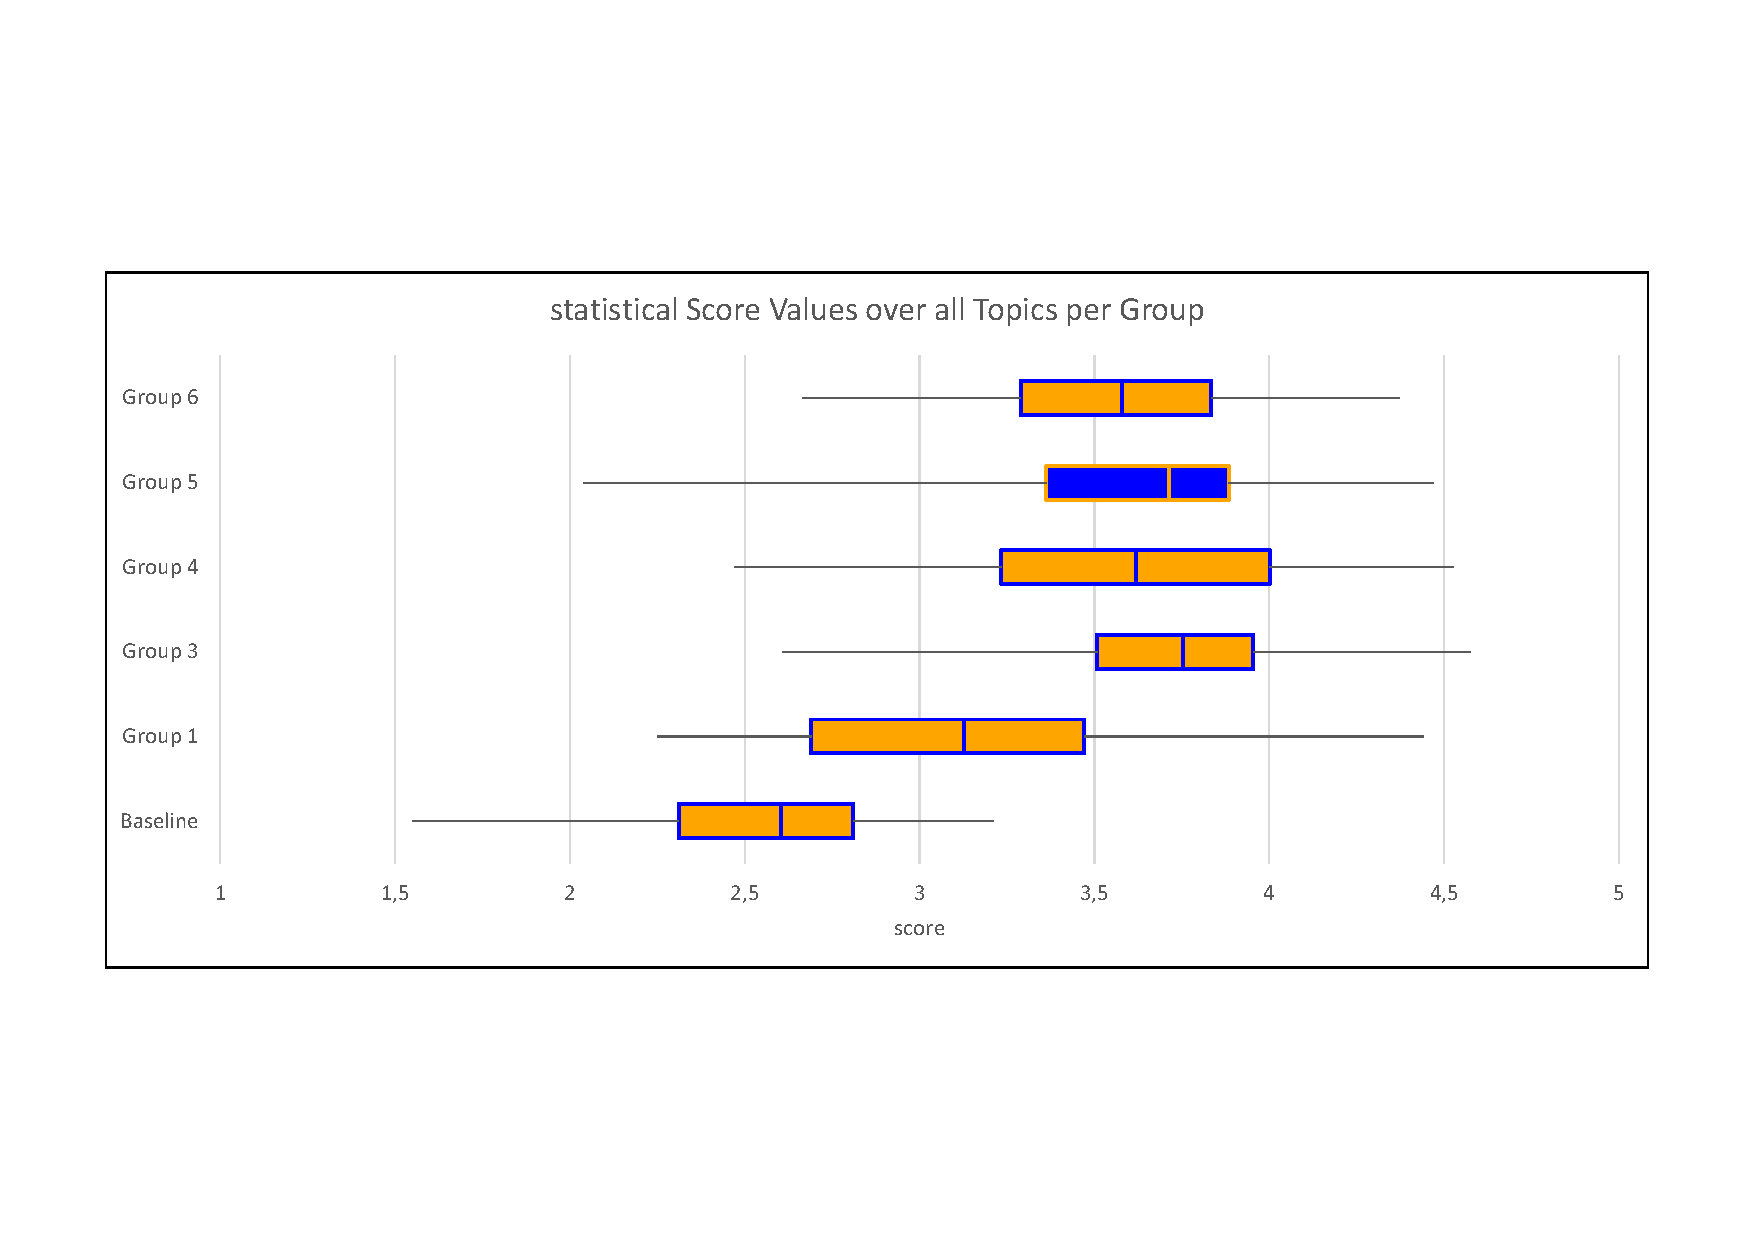
\includegraphics[trim=0 150 0 150, width=\textwidth]{img/box.pdf}
	\caption{statistical values over all topics per group}
	\label{fig:svg}
\end{figure}


\subsection{Score Calculation with all scales}

\begin{figure}[H]
	\centering
	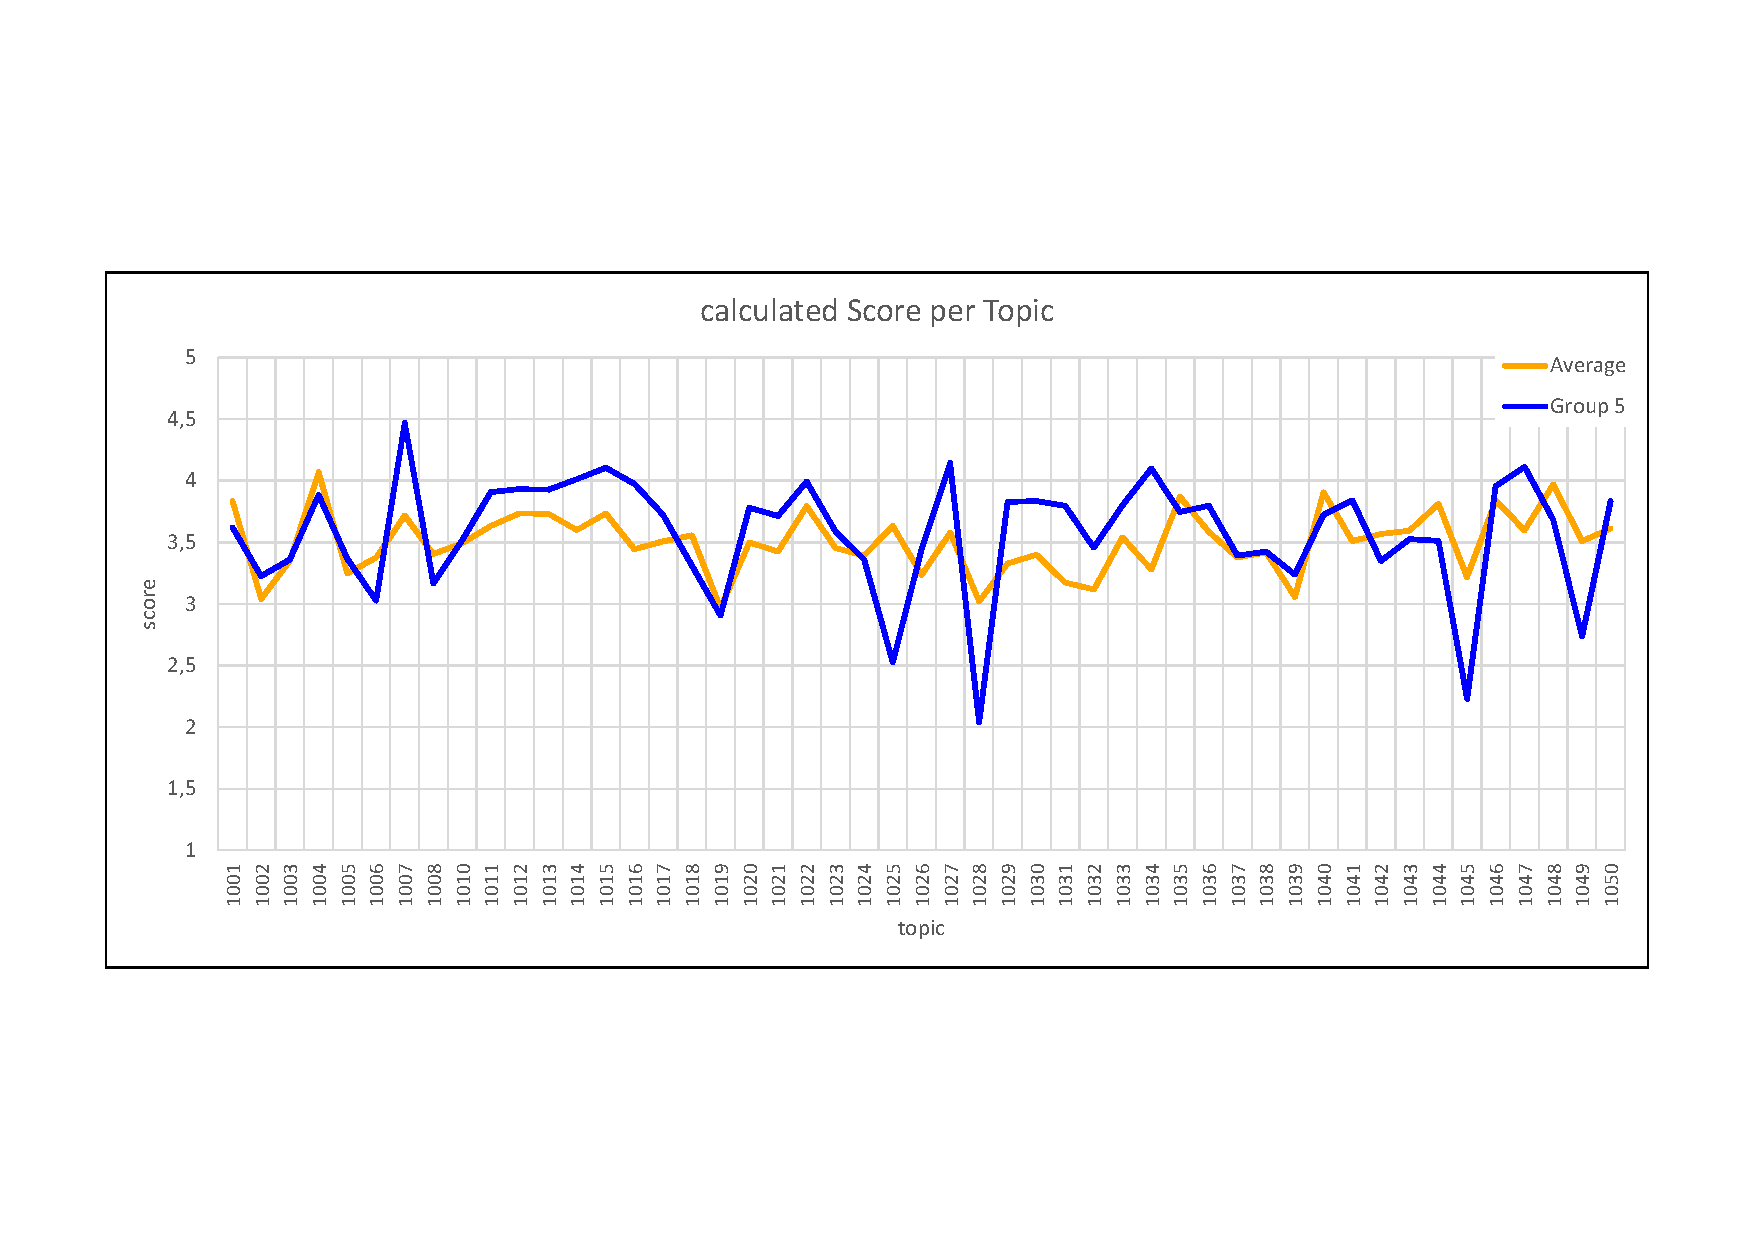
\includegraphics[trim=0 150 0 150, width=\textwidth]{img/score_per_topic.pdf}
	\caption{scores per topic}
	\label{fig:spt}
\end{figure}


\subsection{calculated score per topic - sorted}

\begin{figure}[H]
	\centering
	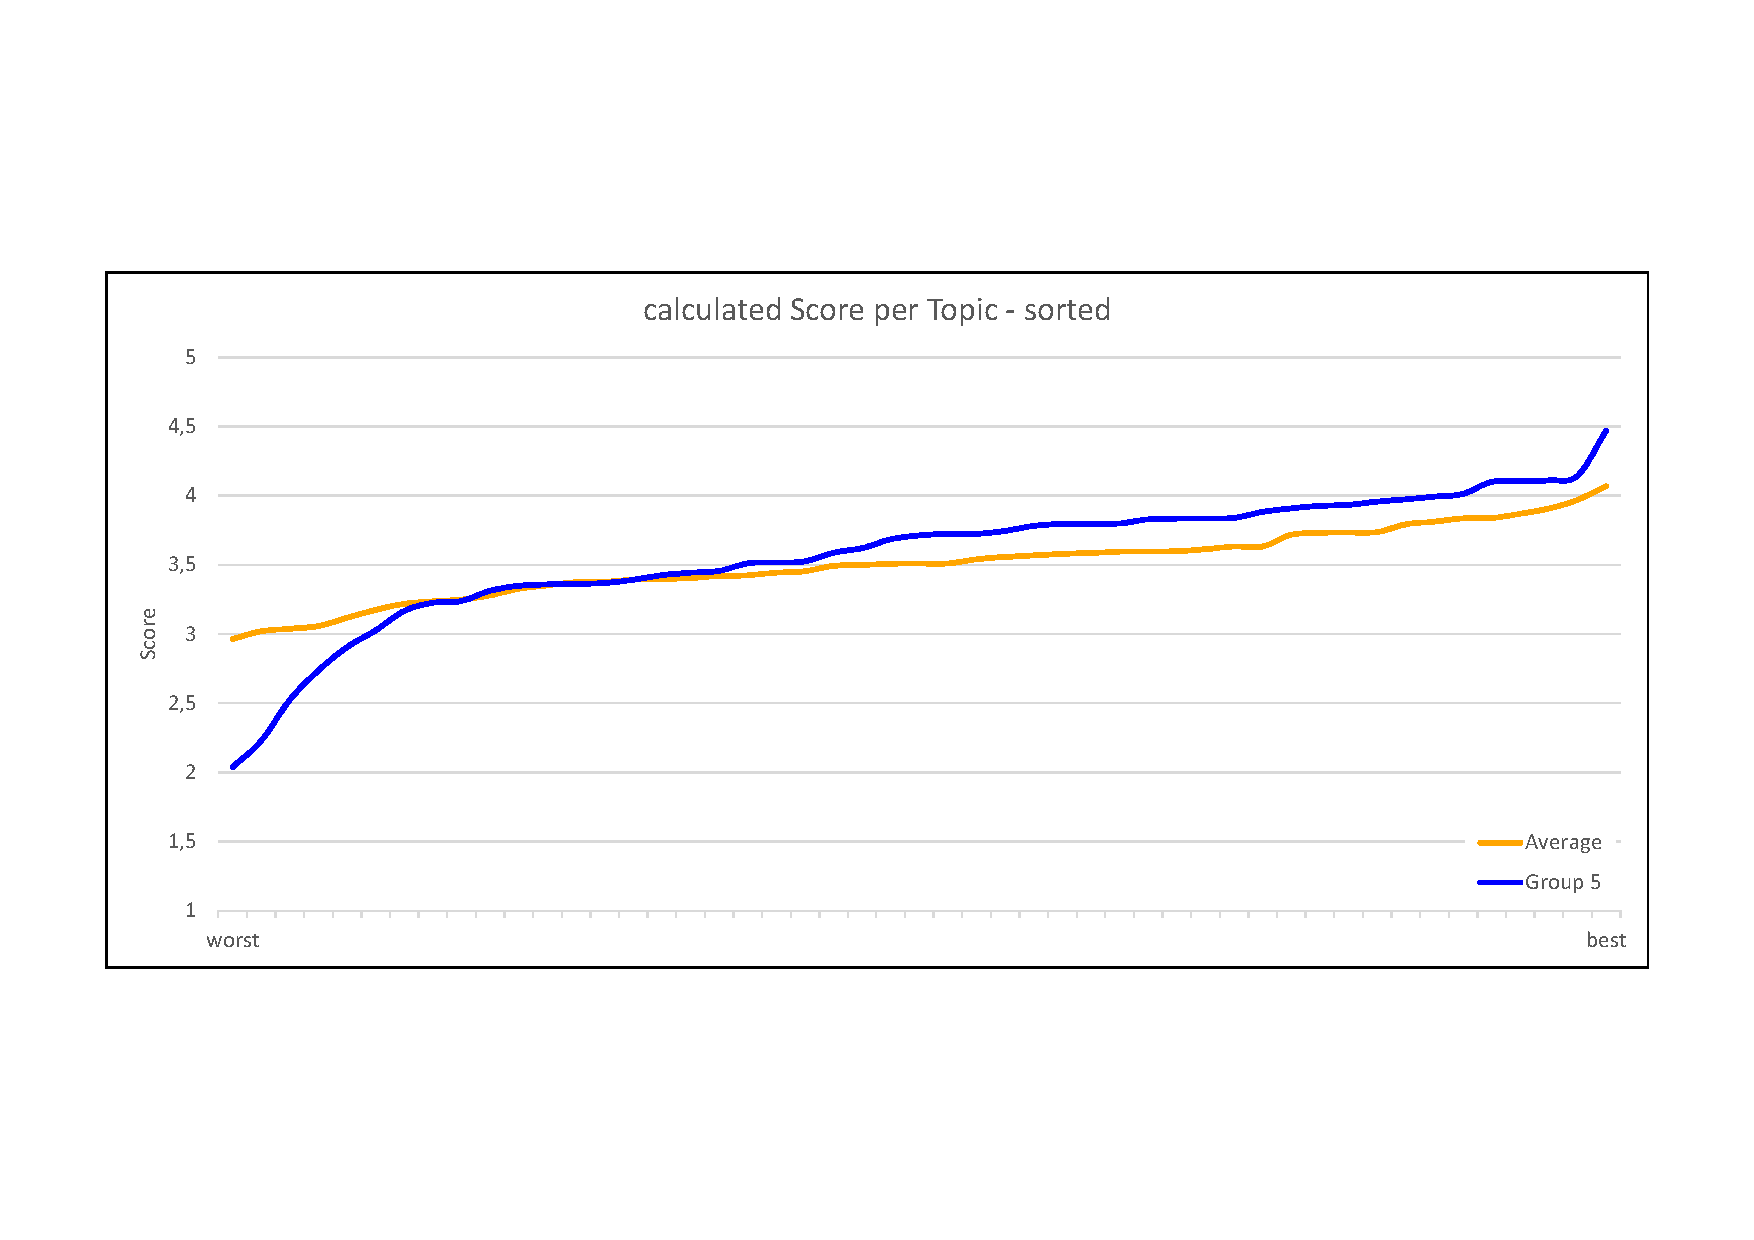
\includegraphics[trim=0 150 0 150, width=\textwidth]{img/score_per_topic_sorted.pdf}
	\caption{scores per topic sorted ascending}
	\label{fig:spts}
\end{figure}

\subsection{best and worst}
	
	\bibliographystyle{plainnat}
	\bibliography{references}

\end{document}

%\begin{abstract}
%  The abstract paragraph should be indented \nicefrac{1}{2}~inch
%  (3~picas) on both the left- and right-hand margins. Use 10~point
%  type, with a vertical spacing (leading) of 11~points.  The word
%  \textbf{Abstract} must be centered, bold, and in point size 12. Two
%  line spaces precede the abstract. The abstract must be limited to
%  one paragraph.
%\end{abstract}
%
%\section{Submission of papers to NIPS 2018}
%
%NIPS requires electronic submissions.  The electronic submission site
%is
%\begin{center}
%  \url{https://cmt.research.microsoft.com/NIPS2018/}
%\end{center}
%
%Please read the instructions below carefully and follow them faithfully.
%
%\subsection{Style}
%
%Papers to be submitted to NIPS 2018 must be prepared according to the
%instructions presented here. Papers may only be up to eight pages
%long, including figures. Additional pages \emph{containing only
%  acknowledgments and/or cited references} are allowed. Papers that
%exceed eight pages of content (ignoring references) will not be
%reviewed, or in any other way considered for presentation at the
%conference.
%
%The margins in 2018 are the same as since 2007, which allow for
%$\sim$$15\%$ more words in the paper compared to earlier years.
%
%Authors are required to use the NIPS \LaTeX{} style files obtainable
%at the NIPS website as indicated below. Please make sure you use the
%current files and not previous versions. Tweaking the style files may
%be grounds for rejection.
%
%\subsection{Retrieval of style files}
%
%The style files for NIPS and other conference information are
%available on the World Wide Web at
%\begin{center}
%  \url{http://www.nips.cc/}
%\end{center}
%The file \verb+nips_2018.pdf+ contains these instructions and
%illustrates the various formatting requirements your NIPS paper must
%satisfy.
%
%The only supported style file for NIPS 2018 is \verb+nips_2018.sty+,
%rewritten for \LaTeXe{}.  \textbf{Previous style files for \LaTeX{}
%  2.09, Microsoft Word, and RTF are no longer supported!}
%
%The \LaTeX{} style file contains three optional arguments: \verb+final+,
%which creates a camera-ready copy, \verb+preprint+, which creates a
%preprint for submission to, e.g., arXiv, and \verb+nonatbib+, which will
%not load the \verb+natbib+ package for you in case of package clash.
%
%\paragraph{New preprint option for 2018}
%If you wish to post a preprint of your work online, e.g., on arXiv,
%using the NIPS style, please use the \verb+preprint+ option. This will
%create a nonanonymized version of your work with the text
%``Preprint. Work in progress.''  in the footer. This version may be
%distributed as you see fit. Please \textbf{do not} use the
%\verb+final+ option, which should \textbf{only} be used for papers
%accepted to NIPS.
%
%At submission time, please omit the \verb+final+ and \verb+preprint+
%options. This will anonymize your submission and add line numbers to aid
%review. Please do \emph{not} refer to these line numbers in your paper
%as they will be removed during generation of camera-ready copies.
%
%The file \verb+nips_2018.tex+ may be used as a ``shell'' for writing
%your paper. All you have to do is replace the author, title, abstract,
%and text of the paper with your own.
%
%The formatting instructions contained in these style files are
%summarized in Sections \ref{gen_inst}, \ref{headings}, and
%\ref{others} below.
%
%\section{General formatting instructions}
%\label{gen_inst}
%
%The text must be confined within a rectangle 5.5~inches (33~picas)
%wide and 9~inches (54~picas) long. The left margin is 1.5~inch
%(9~picas).  Use 10~point type with a vertical spacing (leading) of
%11~points.  Times New Roman is the preferred typeface throughout, and
%will be selected for you by default.  Paragraphs are separated by
%\nicefrac{1}{2}~line space (5.5 points), with no indentation.
%
%The paper title should be 17~point, initial caps/lower case, bold,
%centered between two horizontal rules. The top rule should be 4~points
%thick and the bottom rule should be 1~point thick. Allow
%\nicefrac{1}{4}~inch space above and below the title to rules. All
%pages should start at 1~inch (6~picas) from the top of the page.
%
%For the final version, authors' names are set in boldface, and each
%name is centered above the corresponding address. The lead author's
%name is to be listed first (left-most), and the co-authors' names (if
%different address) are set to follow. If there is only one co-author,
%list both author and co-author side by side.
%
%Please pay special attention to the instructions in Section \ref{others}
%regarding figures, tables, acknowledgments, and references.
%
%\section{Headings: first level}
%\label{headings}
%
%All headings should be lower case (except for first word and proper
%nouns), flush left, and bold.
%
%First-level headings should be in 12-point type.
%
%\subsection{Headings: second level}
%
%Second-level headings should be in 10-point type.
%
%\subsubsection{Headings: third level}
%
%Third-level headings should be in 10-point type.
%
%\paragraph{Paragraphs}
%
%There is also a \verb+\paragraph+ command available, which sets the
%heading in bold, flush left, and inline with the text, with the
%heading followed by 1\,em of space.
%
%\section{Citations, figures, tables, references}
%\label{others}
%
%These instructions apply to everyone.
%
%\subsection{Citations within the text}
%
%The \verb+natbib+ package will be loaded for you by default.
%Citations may be author/year or numeric, as long as you maintain
%internal consistency.  As to the format of the references themselves,
%any style is acceptable as long as it is used consistently.
%
%The documentation for \verb+natbib+ may be found at
%\begin{center}
%  \url{http://mirrors.ctan.org/macros/latex/contrib/natbib/natnotes.pdf}
%\end{center}
%Of note is the command \verb+\citet+, which produces citations
%appropriate for use in inline text.  For example,
%\begin{verbatim}
%   \citet{hasselmo} investigated\dots
%\end{verbatim}
%produces
%\begin{quote}
%  Hasselmo, et al.\ (1995) investigated\dots
%\end{quote}
%
%If you wish to load the \verb+natbib+ package with options, you may
%add the following before loading the \verb+nips_2018+ package:
%\begin{verbatim}
%   \PassOptionsToPackage{options}{natbib}
%\end{verbatim}
%
%If \verb+natbib+ clashes with another package you load, you can add
%the optional argument \verb+nonatbib+ when loading the style file:
%\begin{verbatim}
%   \usepackage[nonatbib]{nips_2018}
%\end{verbatim}
%
%As submission is double blind, refer to your own published work in the
%third person. That is, use ``In the previous work of Jones et
%al.\ [4],'' not ``In our previous work [4].'' If you cite your other
%papers that are not widely available (e.g., a journal paper under
%review), use anonymous author names in the citation, e.g., an author
%of the form ``A.\ Anonymous.''
%
%\subsection{Footnotes}
%
%Footnotes should be used sparingly.  If you do require a footnote,
%indicate footnotes with a number\footnote{Sample of the first
%  footnote.} in the text. Place the footnotes at the bottom of the
%page on which they appear.  Precede the footnote with a horizontal
%rule of 2~inches (12~picas).
%
%Note that footnotes are properly typeset \emph{after} punctuation
%marks.\footnote{As in this example.}
%
%\subsection{Figures}
%
%\begin{figure}
%  \centering
%  \fbox{\rule[-.5cm]{0cm}{4cm} \rule[-.5cm]{4cm}{0cm}}
%  \caption{Sample figure caption.}
%\end{figure}
%
%All artwork must be neat, clean, and legible. Lines should be dark
%enough for purposes of reproduction. The figure number and caption
%always appear after the figure. Place one line space before the figure
%caption and one line space after the figure. The figure caption should
%be lower case (except for first word and proper nouns); figures are
%numbered consecutively.
%
%You may use color figures.  However, it is best for the figure
%captions and the paper body to be legible if the paper is printed in
%either black/white or in color.
%
%\subsection{Tables}
%
%All tables must be centered, neat, clean and legible.  The table
%number and title always appear before the table.  See
%Table~\ref{sample-table}.
%
%Place one line space before the table title, one line space after the
%table title, and one line space after the table. The table title must
%be lower case (except for first word and proper nouns); tables are
%numbered consecutively.
%
%Note that publication-quality tables \emph{do not contain vertical
%  rules.} We strongly suggest the use of the \verb+booktabs+ package,
%which allows for typesetting high-quality, professional tables:
%\begin{center}
%  \url{https://www.ctan.org/pkg/booktabs}
%\end{center}
%This package was used to typeset Table~\ref{sample-table}.
%
%\begin{table}
%  \caption{Sample table title}
%  \label{sample-table}
%  \centering
%  \begin{tabular}{lll}
%    \toprule
%    \multicolumn{2}{c}{Part}                   \\
%    \cmidrule(r){1-2}
%    Name     & Description     & Size ($\mu$m) \\
%    \midrule
%    Dendrite & Input terminal  & $\sim$100     \\
%    Axon     & Output terminal & $\sim$10      \\
%    Soma     & Cell body       & up to $10^6$  \\
%    \bottomrule
%  \end{tabular}
%\end{table}
%
%\section{Final instructions}
%
%Do not change any aspects of the formatting parameters in the style
%files.  In particular, do not modify the width or length of the
%rectangle the text should fit into, and do not change font sizes
%(except perhaps in the \textbf{References} section; see below). Please
%note that pages should be numbered.
%
%\section{Preparing PDF files}
%
%Please prepare submission files with paper size ``US Letter,'' and
%not, for example, ``A4.''
%
%Fonts were the main cause of problems in the past years. Your PDF file
%must only contain Type 1 or Embedded TrueType fonts. Here are a few
%instructions to achieve this.
%
%\begin{itemize}
%
%\item You should directly generate PDF files using \verb+pdflatex+.
%
%\item You can check which fonts a PDF files uses.  In Acrobat Reader,
%  select the menu Files$>$Document Properties$>$Fonts and select Show
%  All Fonts. You can also use the program \verb+pdffonts+ which comes
%  with \verb+xpdf+ and is available out-of-the-box on most Linux
%  machines.
%
%\item The IEEE has recommendations for generating PDF files whose
%  fonts are also acceptable for NIPS. Please see
%  \url{http://www.emfield.org/icuwb2010/downloads/IEEE-PDF-SpecV32.pdf}
%
%\item \verb+xfig+ "patterned" shapes are implemented with bitmap
%  fonts.  Use "solid" shapes instead.
%
%\item The \verb+\bbold+ package almost always uses bitmap fonts.  You
%  should use the equivalent AMS Fonts:
%\begin{verbatim}
%   \usepackage{amsfonts}
%\end{verbatim}
%followed by, e.g., \verb+\mathbb{R}+, \verb+\mathbb{N}+, or
%\verb+\mathbb{C}+ for $\mathbb{R}$, $\mathbb{N}$ or $\mathbb{C}$.  You
%can also use the following workaround for reals, natural and complex:
%\begin{verbatim}
%   \newcommand{\RR}{I\!\!R} %real numbers
%   \newcommand{\Nat}{I\!\!N} %natural numbers
%   \newcommand{\CC}{I\!\!\!\!C} %complex numbers
%\end{verbatim}
%Note that \verb+amsfonts+ is automatically loaded by the
%\verb+amssymb+ package.
%
%\end{itemize}
%
%If your file contains type 3 fonts or non embedded TrueType fonts, we
%will ask you to fix it.
%
%\subsection{Margins in \LaTeX{}}
%
%Most of the margin problems come from figures positioned by hand using
%\verb+\special+ or other commands. We suggest using the command
%\verb+\includegraphics+ from the \verb+graphicx+ package. Always
%specify the figure width as a multiple of the line width as in the
%example below:
%\begin{verbatim}
%   \usepackage[pdftex]{graphicx} ...
%   \includegraphics[width=0.8\linewidth]{myfile.pdf}
%\end{verbatim}
%See Section 4.4 in the graphics bundle documentation
%(\url{http://mirrors.ctan.org/macros/latex/required/graphics/grfguide.pdf})
%
%A number of width problems arise when \LaTeX{} cannot properly
%hyphenate a line. Please give LaTeX hyphenation hints using the
%\verb+\-+ command when necessary.
%
%\subsubsection*{Acknowledgments}
%
%Use unnumbered third level headings for the acknowledgments. All
%acknowledgments go at the end of the paper. Do not include
%acknowledgments in the anonymized submission, only in the final paper.
%
%\section*{References}
%
%References follow the acknowledgments. Use unnumbered first-level
%heading for the references. Any choice of citation style is acceptable
%as long as you are consistent. It is permissible to reduce the font
%size to \verb+small+ (9 point) when listing the references. {\bf
%  Remember that you can use more than eight pages as long as the
%  additional pages contain \emph{only} cited references.}
%\medskip
%
%\small
%
%[1] Alexander, J.A.\ \& Mozer, M.C.\ (1995) Template-based algorithms
%for connectionist rule extraction. In G.\ Tesauro, D.S.\ Touretzky and
%T.K.\ Leen (eds.), {\it Advances in Neural Information Processing
%  Systems 7}, pp.\ 609--616. Cambridge, MA: MIT Press.
%
%[2] Bower, J.M.\ \& Beeman, D.\ (1995) {\it The Book of GENESIS:
%  Exploring Realistic Neural Models with the GEneral NEural SImulation
%  System.}  New York: TELOS/Springer--Verlag.
%
%[3] Hasselmo, M.E., Schnell, E.\ \& Barkai, E.\ (1995) Dynamics of
%learning and recall at excitatory recurrent synapses and cholinergic
%modulation in rat hippocampal region CA3. {\it Journal of
%  Neuroscience} {\bf 15}(7):5249-5262.
